%%%%%%%%%%%%%%%%%%%%%%%%%%%%%%%%%%%%%%%%%%%%%%%%%%%%%%%%%%%%%%%%%%%%%
%% I, the copyright holder of this work, release this work into the
%% public domain. This applies worldwide. In some countries this may
%% not be legally possible; if so: I grant anyone the right to use
%% this work for any purpose, without any conditions, unless such
%% conditions are required by law.
%%%%%%%%%%%%%%%%%%%%%%%%%%%%%%%%%%%%%%%%%%%%%%%%%%%%%%%%%%%%%%%%%%%%%

\PassOptionsToPackage{
  plainpages = false,               								
  pdfpagelabels,
  unicode,  
  colorlinks = true,
  linkcolor = link-grey,	% PC version
  citecolor = crimson,		% PC version
  urlcolor = blue,			% PC version
  % linkcolor = black,		% Print version
  % citecolor = black,		% Print version
  % urlcolor = black,		% Print version
}{hyperref}

\documentclass[
  digital,  	% PC version
  color,		% PC version
  oneside,   	% PC version
  % printed 	% Printed version
  % monochrome	% Printed version
  % twoside		% Printed version
  12pt,
  nocover,
  notable,
  nolof,
  nolot,
  %% More options are listed in the user guide at
  %% <http://mirrors.ctan.org/macros/latex/contrib/fithesis/guide/mu/fi.pdf>.
]{fithesis3}

%% The following section sets up the locales used in the thesis.
\usepackage[resetfonts]{cmap} %% We need to load the T2A font encoding
\usepackage[utf8]{inputenc}
\usepackage[T1,T2A]{fontenc}  %% to use the Cyrillic fonts with Russian texts.
\usepackage[
  main=english,
  english, german, russian, czech, slovak
]{babel}
%% fonts:
\usepackage{paratype}
\def\textrussian#1{{\usefont{T2A}{PTSerif-TLF}{m}{rm}#1}}

%%\shorthands{off}
%% The following section sets up the metadata of the thesis.
\thesissetup{
    date          = \the\year/\the\month/\the\day,
    university    = mu,
    faculty       = fi,
    type          = mgr,
    author        = Ľubomír Obrátil,
    gender        = m,
    advisor       = {RNDr. Petr Švenda, Ph.D.},
    title         = {Randomness Testing Toolkit},
    TeXtitle      = {The automated testing of randomness with multiple statistical batteries},
    keywords      = {TODO},
    TeXkeywords   = {TODO},
    abstract      = {TODO},
    thanks        = {TODO},
    bib           = bibliography.bib,
}
\usepackage{makeidx}      %% The `makeidx` package contains
\makeindex                %% helper commands for index typesetting.
\thesisload


\newcommand{\lmar}{3.6cm} % PC
\newcommand{\rmar}{3.6cm} % PC
%\newcommand{\lmar}{4cm} % Printed
%\newcommand{\rmar}{3.2cm} % Printed

\usepackage[top=3cm, bottom=3.5cm, left=\lmar, right=\rmar]{geometry}

%% These additional packages are used within the document:\\
\usepackage{booktabs}
\usepackage{minted}
\usepackage{paralist} %% Compact list environments
\usepackage{amsmath}  %% Mathematics
\usepackage{amsthm}
\usepackage{url}
\usepackage{enumitem}
\usepackage{amsfonts}
\usepackage{markdown} %% Lightweight markup
\usepackage{dirtree}
\usepackage{amssymb}
\usepackage{colortbl}
\usepackage{rotating} 

\usepackage{makecell}
\renewcommand\theadfont{\bfseries}

\usepackage{siunitx}
\sisetup{output-exponent-marker=\ensuremath{\mathrm{e}}}

\usepackage{xcolor}
\definecolor{link-grey}{rgb}{0.3,0.3,0.3}
\definecolor{code-bg-grey}{rgb}{0.85,0.85,0.85}
\definecolor{code-bg-light_grey}{rgb}{0.92,0.92,0.92}
\definecolor{crimson}{rgb}{0.6,0,0}
\definecolor{lvl1}{rgb}{0.13,0.51,0.26}
\definecolor{lvl2}{rgb}{0.46,0.77,0.44}
\definecolor{lvl3}{rgb}{0.75,0.9,0.6}
\definecolor{lvl4}{rgb}{1,1,0.8}

\newcommand{\gr}{\cellcolor{green!40}}
\newcommand{\rd}{\cellcolor{red!40}}
\newcommand{\cone}{\cellcolor{lvl1}}
\newcommand{\ctwo}{\cellcolor{lvl2}}
\newcommand{\cthree}{\cellcolor{lvl3}}
\newcommand{\cfour}{\cellcolor{lvl4}}


% Because czech and slovak breaks it...
\begingroup
    \makeatletter
    \catcode`\-=\active
    \AtBeginDocument{
    \def\@@@cmidrule[#1-#2]#3#4{\global\@cmidla#1\relax
        \global\advance\@cmidla\m@ne
        \ifnum\@cmidla>0\global\let\@gtempa\@cmidrulea\else
        \global\let\@gtempa\@cmidruleb\fi
        \global\@cmidlb#2\relax
        \global\advance\@cmidlb-\@cmidla
        \global\@thisrulewidth=#3
        \@setrulekerning{#4}
        \ifnum\@lastruleclass=\z@\vskip \aboverulesep\fi
        \ifnum0=`{\fi}\@gtempa
        \noalign{\ifnum0=`}\fi\futurenonspacelet\@tempa\@xcmidrule}
    }
\endgroup

% Eliminates margins
\def\nomar{\list{}{\rightmargin-\rmar\leftmargin-\lmar}\item[]}
\let\endnomar=\endlist

% Rotates table cell
\newcolumntype{R}[1]{>{\begin{turn}{90}\begin{minipage}{#1}}l%
<{\end{minipage}\end{turn}}%
}

% Various macros
\setlength{\parskip}{0.5em}
\setlist[description]{leftmargin=0cm , itemsep = 0cm}
\setlist[itemize]{noitemsep}

% Itemize with title
\newenvironment{titlemize}[1]
{
	\begin{description}
	\item[#1]\
	\begin{itemize}
}
{
	\end{itemize}
 	\end{description}
}

\newtheorem{theorem}{Theorem}[section]
\newtheorem{corollary}{Corollary}[theorem]
\newtheorem{lemma}[theorem]{Lemma}

\theoremstyle{definition}
\newtheorem{definition}{Definition}[section]
\newtheorem{conjecture}{Conjecture}[section]
\newtheorem{example}{Example}[section]

\theoremstyle{remark}
\newtheorem*{rem}{Remark}
\newtheorem*{note}{Note}

% Let tables and figures share numbering
\makeatletter \let\c@table\c@figure \makeatother

\AtBeginEnvironment{minted}{%
  \renewcommand{\fcolorbox}[4][]{#4}}

%%%%%%%%%%%%%%%%%%%%%%%%%%%%%%%%%%%%%%%%%%%%%%%%%%%%%%%%%%%%%%%%%%%%%%%%%%%%%%%%%%%%%%%%
%%%%%%%%%%%%%%%%%%%%%%%%%%%%%%%%%%%%%%%%%%%%%%%%%%%%%%%%%%%%%%%%%%%%%%%%%%%%%%%%%%%%%%%%
% =================================== TEXT BEGINNING =================================== 
%%%%%%%%%%%%%%%%%%%%%%%%%%%%%%%%%%%%%%%%%%%%%%%%%%%%%%%%%%%%%%%%%%%%%%%%%%%%%%%%%%%%%%%%
%%%%%%%%%%%%%%%%%%%%%%%%%%%%%%%%%%%%%%%%%%%%%%%%%%%%%%%%%%%%%%%%%%%%%%%%%%%%%%%%%%%%%%%%
% Final Description:
%The randomness and pseudorandomness are important security property of output of a random number generator as well a cryptographic function. To some extent, these characteristics can be measured and tested by randomness statistical batteries like STS NIST or DIEHARDER. The thesis is aimed at development of a tool that would provide means for fast, simple and consistent testing of randomness of arbitrary data using multiple statistical batteries.

%The thesis will provide an introduction to statistical randomness testing and interpretation of results obtained from a given test and battery. The toolkit for easy remote execution of statistical tests on a dedicated server will be developed with the following functionality:

% - Easy submission of data for testing, both locally (filesystem) and remotely (web interface)
% - At least three different statistical batteries will be incorporated via unified interface
% - Unified presentation of test results of executed batteries
%The tool will be utilized in subsequent experiments aimed to compare classical batteries with EACirc framework and also evaluate test behavior of DIEHARDER on large amount of truly random data.

%Literature
%STS NIST battery, http://csrc.nist.gov/groups/ST/toolkit/rng/index.html [2017-03-13]
%R. Brown, Dieharder battery, https://www.phy.duke.edu/~rgb/General/dieharder.php[2017-03-13]

\begin{document}

\chapter{Introduction}
\begin{itemize}
\item Randomness, why should we test it (defects, low entropy, etc...)
\item Statistical testing of randomness
\end{itemize}

\chapter{Used third-party statistical software}
\label{chap:batteries}
In this chapter, we will explain terminology specific to Randomness Testing Toolkit; present a quick overview of the statistical software used in the toolkit and describe the observed and unexpected behavior of the statistical software in edge cases. We also list undertaken measures to mitigate the undocumented behaviour in our further experiments.

\section{Terminology}
Throughout the thesis, we are using certain expressions in the context of Randomness Testing Toolkit and the tools and math it uses. We list these terms along with their explanations here.

\begin{description}
\item[(Statistical) Battery] \hfill \\
A program developed by a third party serving as a tool for evaluation of randomness of arbitrary binary data. A statistical battery usually contains one or more statistical tests. The final result of the assessment is based on the results of the tests. Examples of statistical batteries are NIST Statistical Test Suite, Dieharder or TestU01.

\item[(Statistical) Test] \hfill \\
A single unit in statistical battery that measures some property of the tested binary stream (e.g. number of zeroes). The test can have multiple variants and subtests, and the result of the test is one or multiple statistics.

\item[Null hypothesis - $H_0$] \hfill \\
The hypothesis $H_0$ denotes the hypothesis that the tested data stream is random. Based on the results of the test, we can either reject $H_0$ and say that the data are not random or not reject it. In the latter case, we assume that the tested data are indeed random.

\item[P-value] \hfill \\
In our hypothesis testing, a p-value is a probability of obtaining equal or more extreme test result while $H_0$ holds true. In our situation, a p-value denotes the probability that we would get same or more extreme test results when testing truly random data. Therefore, the closer the p-value is to 0 the less is the probability the tested data is random and vice versa.

\item[Alpha - $\alpha$] \hfill \\
Significance level based on which we either reject or not reject $H_0$. We can specify some interval (e.g. $[0,\alpha]$) and if the result of the test (p-value) falls into this interval, we will reject the hypothesis that the tested data is random. Alternatively, we can also reject p-values that are too extreme on both sides of the interval (outside of $\left[\frac{\alpha}{2},1-\frac{\alpha}{2}\right]$).

\item[Type I and type II errors] \hfill \\
A type I error (false positive) is the rejection of a true null hypothesis $H_0$. On the opposite, a type II error (false negative) is incorrectly holding to the null hypothesis, even when it should have been rejected.

\item[Statistic] \hfill \\
The value obtained by certain calculation from first level p-values. Multiple statistics can be obtained from one set of p-values e.g. when testing the set for uniformity we can use Kolmogorov-Smirnov Test or Chi-Square test. Based on values of statistics of a test we can decide rejection of $H_0$.

\item[Test sample] \hfill \\
A single execution of a statistical test. The result of single test execution is one first level p-value. By repeating execution of the test, we obtain multiple p-values. By using a certain statistic (e.g. Kolmogorov-Smirnov test), we can calculate a single second level p-value.

\item[Variant of a test] \hfill \\
Many tests can be parametrized in some ways, possibly giving different results with the same input data. We don't treat multiple executions of a single test with different settings as separate units but rather as variants of that test.

\item[Subtest] \hfill \\
Some tests, even when executed only once, may measure multiple properties of the data thus providing multiple results. For example, Serial Test from Dieharder battery will measure frequencies of all 1, 2, .., 16-bit patterns in the data. We treat these measurements separately - as subtests of the test. The subtests can have multiple separate statistics.

\item[Job] \hfill \\
Single execution of Randomness Testing Toolkit that will analyse single binary data file with single statistical battery.

\item[Experiment] \hfill \\
Batch of jobs that analysed single data file with various statistical batteries and settings.

\end{description}

\section{Batteries supported by RTT}
\subsection{NIST Statistical Test Suite}
The battery of statistical tests was developed by National Institute of Standards and Technology (cit.). The battery implements 15 statistical tests for evaluating randomness of input data. The tests are listed in Appendix~\ref{app:nist_sts_tests}.

The reference implementation is not used in RTT because it is considerably slower than its optimized counterparts. The faster implementation called NIST STS optimised v5.0.2 used in RTT was developed by Zdeněk Říha and Marek Sýs(cit.).

\subsection{Dieharder}
Dieharder is a battery designed by Robert G. Brown at the Duke University (cit.). The battery features user-friendly console interface with the possibility of fine-grain modification of the test parameters. The fact that Dieharder is included in repositories of some Linux distributions (cit manpage) adds to its popularity and ease of use. Dieharder includes all tests from the older statistical battery Diehard (cit.), three tests from NIST STS and several other tests implemented by the author. The tests, along with their default settings, are listed in Appendix~\ref{app:dieharder_tests}.

Since the original Dieharder implementation doesn't output all of the information we needed for interpretation and evaluation of the results, we had to modify the source code of the battery. RTT uses this modified Dieharder. We modified Dieharder v3.31.1 which is the last stable maintained release on the project page.

\subsection{TestU01}
This library of statistical batteries was developed at Université de Montréal by Pierre L’Ecuyer et al. (cit.). It contains a wide range of tests from NIST STS, Dieharder, and literature. It also implements various pseudo-random number generators. The statistical tests are grouped into multiple categories each intended for different use-case scenario. We will treat these categories of tests as separate batteries. TestU01 includes following ten batteries. The tests included in specific batteries are listed in TestU01 documentation(cit.).

\begin{description}
\item[Small Crush, Crush, Big Crush] \hfill \\
Small Crush battery is very fast and needs a relatively small amount of data to run - around 250 megabytes. Small Crush is also the only battery that can be natively used for analysis of data in a binary file, for the use of Crush and Big Crush, the user has to implement PRNG with the TestU01 interface. Crush and Big Crush batteries are more stringent and need gigabytes of data and a few hours to finish while Big Crush is more time and data demanding.
\item[Rabbit, Alphabit, Block Alphabit] \hfill \\
Tests in these batteries are suited for testing hardware bit generators and can be applied to an arbitrary amount of data. Data can be provided either as a binary file or PRNG implementing the TestU01 interface.
\item[PseudoDIEHARD, FIPS\_140\_2] \hfill \\
Tests in PseudoDIEHARD imitate DIEHARD battery; FIPS\_140\_2 battery implements a small suite of tests in NIST standard(cit.) Randomness Testing Toolkit doesn't support these two batteries since they are subsets of other batteries.
\end{description}

Since TestU01 v1.2.3 is available only as an ANSI C library, we developed a console interface for it. The interface implements a dummy number generator that provides data from a supplied binary file to the battery. Our interface allows us to apply batteries to arbitrary binary data even when the batteries themselves don't support this feature natively.

\section{Unexpected behavior and errors of the batteries}
To examine the boundary behavior of the above-listed tools, we used them to process extremely non-random data streams. The data streams that we used as the input to the batteries were two binary data files consisting of only zeroes and ones respectively. The settings of the batteries remained set to default. 

Below we list observed undocumented behavior that differs from the execution of the batteries with non-extreme input.

\subsection*{NIST Statistical Test Suite}
Each test in the battery processed 1000 separate data streams. Each data stream was 1000000 bits long.

Tests Random Excursions and Random Excursions Variant are not applicable to all possible data streams. In a regular run with reasonably random data, this doesn't matter much, as the tests are repeated multiple times, and the final result will simply be calculated from a lesser number of p-values. 

Neither of the tests can be applied to a stream full of zeroes or ones. This causes absence of results when analyzing such data. The user can find out the fact that the tests are not applicable to provided stream after he inspects logs of the program; otherwise, the interpretation of the missing results is left to him.

\subsection*{Dieharder}
When processing extremely non-random data with Dieharder, we observed various erroneous events. The events are summarized in Table~\ref{tab:dieharder_errors}. 

\begin{table}[h!]
\begin{nomar}
\centering
\begin{tabular}{@{}lcc@{}} \toprule
\textbf{Test name}                   & \textbf{Stream of zeroes} & \textbf{Stream of ones} \\ \midrule
STS Runs                             & No result                & No result                \\
DAB Monobit 2 						 & Invalid result           & Invalid result           \\
Diehard Minimum Distance (2D Circle) & Stuck execution          & --                        \\
Diehard 3D Sphere (Minimum Distance) & Stuck execution          & --                        \\
Marsaglia and Tsang GCD              & Stuck execution          & --                        \\
RGB Generalized Minimum Distance     & Stuck execution          & --                        \\
RGB Kolmogorov-Smirnov               & Stuck execution          & --                        \\  
Diehard Craps                        & --                       & Stuck execution          \\
RGB Bit Distribution                 & --                       & Stuck execution          \\ \bottomrule
\end{tabular}
\end{nomar}
\caption{Undocumented behavior of tests in Dieharder battery}
\label{tab:dieharder_errors}
\end{table}

\begin{titlemize}{Observed errors}
\item \textbf{No result} Test didn't provide any p-values that would be used to calculate the final result of the test. The user is not notified of this, and the final result of the test statistic is based on default value (1.0).
\item \textbf{Invalid result} Test provided resulting statistic and there was no indication of error other than that the result was again default value of the statistic (1.0). Following the definition of p-value, the interpretation of such result is that the analyzed stream was almost certainly random. This is obviously not true, as both streams are just repeating ones or zeroes respectively. 
\item \textbf{Stuck execution} Tests froze at a certain point in execution, did not produce any results and we were forced to kill the processes manually.
\end{titlemize}

\subsection*{TestU01}
Batteries Small Crush, Crush, Big Crush, Rabbit, Alphabit and Block Alphabit were executed. Tests that are part of multiple batteries acted in the same way across the batteries. The behavior is summarized in Table~\ref{tab:testu01_errors}.

\begin{table}[h!]
\begin{nomar}
\centering
\begin{tabular}{@{}lcc@{}} \toprule
\textbf{Test name}                 & \textbf{Stream of zeroes} & \textbf{Stream of ones} \\ \midrule    
sstring\_Run                       & No result                & No result                \\
sknuth\_Gap                        & No result                & --                        \\
svaria\_SampleProd                 & All results invalid      & All results invalid      \\
svaria\_AppearenceSpacings         & All results invalid      & All results invalid      \\   
scomp\_LinearComp                  & All results invalid      & All results invalid      \\
scomp\_LempelZiv                   & All results invalid      & All results invalid      \\
svaria\_SampleCorr                 & --                       & All results invalid      \\ 
sknuth\_MaxOft                     & Some results invalid     & Some results invalid     \\
svaria\_SampleMean                 & Some results invalid     & Some results invalid     \\
sspectral\_Fourier3                & Some results invalid     & Some results invalid     \\
sstring\_HammingWeight2            & Some results invalid     & Some results invalid     \\
sstring\_AutoCor                   & Some results invalid     & Some results invalid     \\
smultin\_MultinomialBitsOver       & Some results invalid     & Some results invalid     \\
sstring\_LongestHeadRun            & --                       & Some results invalid     \\
snpair\_ClosePairs                 & Stuck execution          & Stuck execution          \\
snpair\_ClosePairsBitMatch         & --                       & Stuck execution          \\
svaria\_SumCollector               & --                       & Stuck execution          \\
smarsa\_GCD                        & --                       & Stuck execution          \\ \bottomrule                          
\end{tabular}
\end{nomar}  
\caption{Undocumented behavior of tests in TestU01 library}
\label{tab:testu01_errors}                                                                                           
\end{table}

\begin{titlemize}{Observed errors}
\item \textbf{No results} Tests reported warning and ended without any result. This is probably caused by the tests not being applicable to provided data.
\item \textbf{All results invalid}  All statistics of the test reported p-value very close to 1.0. This could lead the user to the interpretation that the test reports the data as an almost perfect random stream.
\item \textbf{Some results invalid} Similar situation to the previous one but not all statistics of the test are close to 1.0. Results of tests statistics are either close to 0.0 or 1.0.
\item \textbf{Stuck execution} Tests froze at a certain point of execution. In some cases, this is preceded by an issued warning. Tests didn't produce any results and had to be killed manually.
\end{titlemize}

\subsection{Preventive measures in RTT}
\label{sec:preventive_measures_rtt}
Since we need to use the batteries in RTT with arbitrary binary data, we implemented following measures that mitigate above-mentioned errors in our experiments.
\begin{itemize}
\item Tests that don't produce any results are ignored and treated as if never executed.
\item Because some tests give 1.0 as a result of their statistics when the data are clearly not random, we will reject the hypothesis of randomness either when the p-value is too close to 0 or is equal to 1. More specifically, $H_0$ will be rejected for all p-values that falls outside of the interval $\left[\alpha, 1\right)$.
\item Each test is executed with the timeout. If the test doesn't finish within defined time limit, we will automatically terminate it and then treat it as if it didn't produce any results.
\end{itemize}

\chapter{Randomness Testing Toolkit}
One of our goals during working on this project was to create a tool that would provide fast and user-friendly analysis of randomness even for users not experienced in the field of statistical randomness testing. Process of statistical testing generally includes finding a suitable tool, installation of said tool, and an execution and interpretaion of the analysis results.

Another motivation was that the developed tool would unite the process of randomness analysis that is often done by researchers in CRoCS\footnote{Centre for Research of Cryptography and Security}. Before the start of the project, each researcher used his own set of scripts and tools to analyse, which is difficult to manage and also complicates comparation of the experiments done by different people.

Therefore we developed Randomness Testing Toolkit\footnote{Also referenced as RTT or just the toolkit.}, a tool that serves as an unified interface of the three statistical batteries presented in Chapter~\ref{chap:batteries}. The toolkit consists of several connected parts that are intended for various purposes. Apart from interfaces and data storage format, the parts are independent and can be exchanged or modified freely.

In the following sections of this chapter, we will provide detailed description of the implemented parts of the toolkit.

\section{Local unified interface}
The local unified interface is at the lowest level of the developed parts of RTT. The interface is a binary executable that accepts settings and outputs the results in common format for all batteries. The executable handles transformation of general settings into the battery specific ones, running the battery executable and then transforming gathered output into general format. The process is visualized in Figure~\ref{fig:rtt_local_workflow}.

The toolkit accepts settings needed for its run from three following sources:
\begin{itemize}
\item \textbf{Command-line arguments} -- Basic settings that can change in every run; e.g. path to input file with binary data or to file with battery configuration.
\item \textbf{Toolkit settings file} -- General settings for the toolkit related to the system environment e.g. paths to executables of the statistical batteries. In most of the cases, the settings stay the same for all executions of the toolkit regardless of the battery or data used. Changes in this configuration are needed only when the environment changes.
\item \textbf{Battery configuration file} -- Configuration file that fully configures input settings for single or multiple batteries. The configuration of the batteries can vary among the executions of the toolkit.
\end{itemize}

\begin{figure}[h!]
\begin{nomar}
\centering
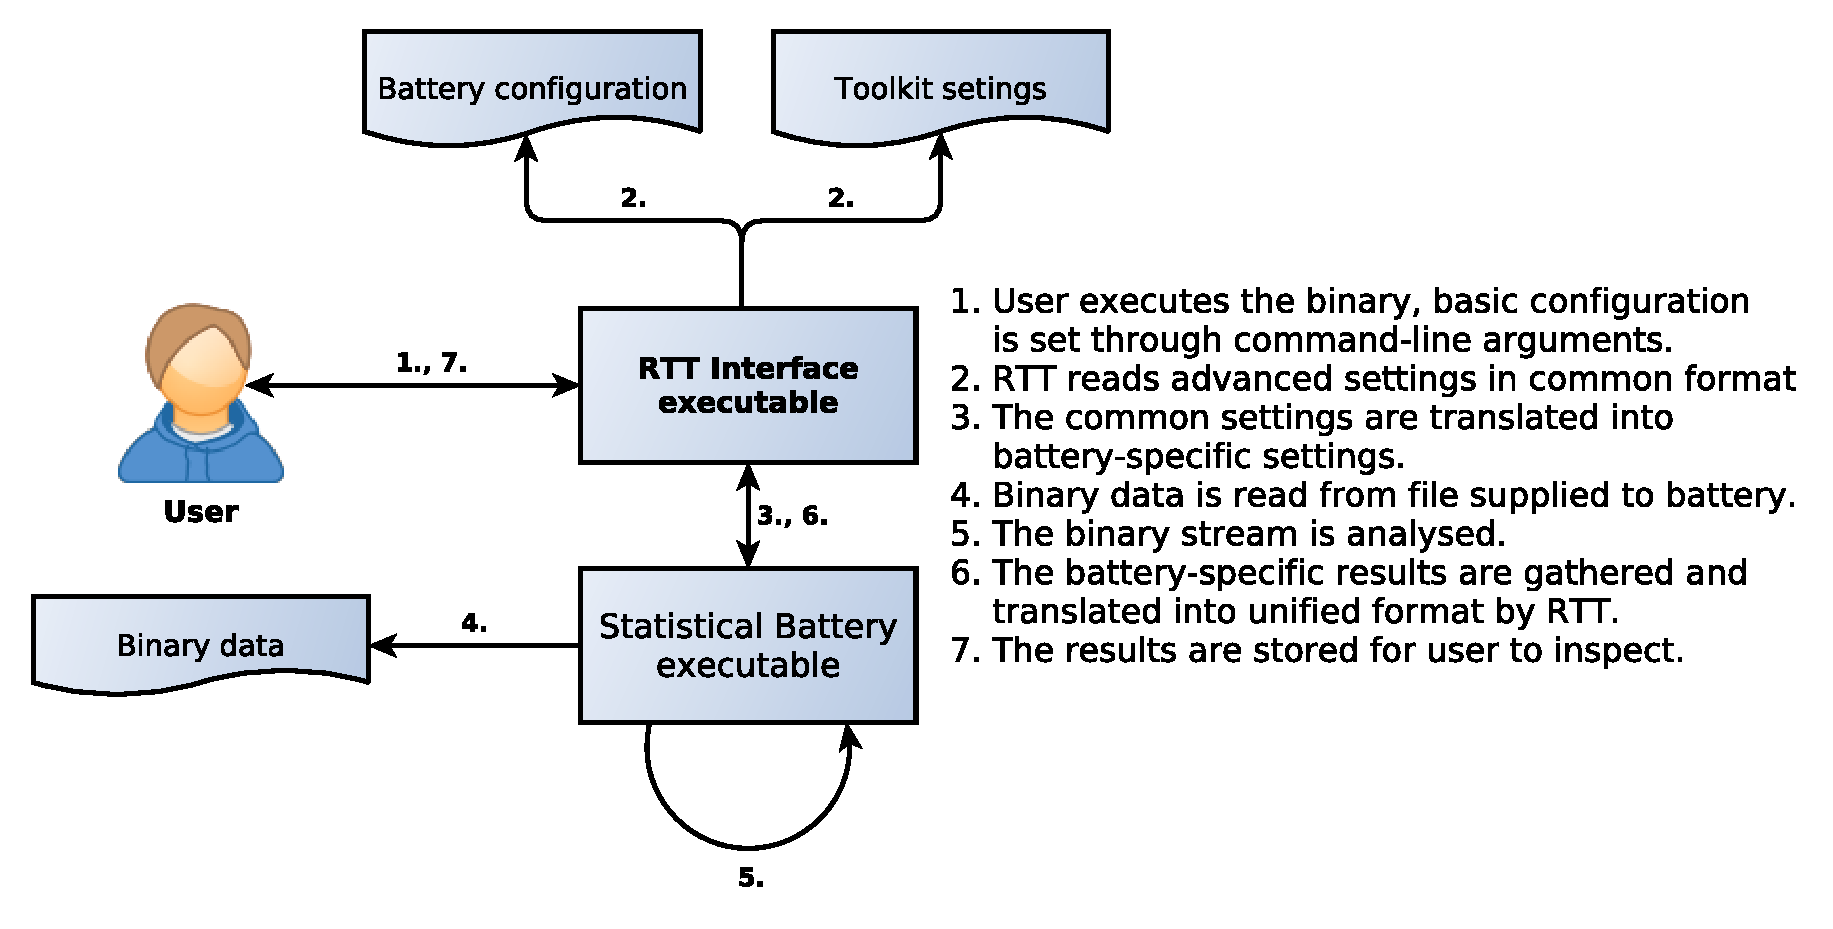
\includegraphics[width=\paperwidth-4cm]{figures/local-rtt-workflow.pdf}
\end{nomar}
\caption{Local RTT workflow}
\label{fig:rtt_local_workflow}
\end{figure}

\subsection{Command-line arguments}
The basic options of the RTT execution are set through command-line arguments. The executable recognizes following options.

\begin{itemize}
\item \texttt{-h} Usage of the toolkit will be printed.
\item \texttt{-b <battery>} Sets the battery that will be executed during the run. Values accepted as \texttt{<battery>}: dieharder, nist\_sts, tu01\_smallcrush, tu01\_crush, tu01\_bigcrush, tu01\_rabbit, tu01\_alphabit and tu01\_block- \linebreak alphabit.
\item \texttt{-t <test-id>} Optional argument. If set, only single test with id \texttt{<test-id>} will be executed in the chosen battery.
\item \texttt{-c <config-path>} Path to file with configuration of the battery. Details about battery configuration are in Section~\ref{sec:batt_conf}.
\item \texttt{-f <data-path>} Path to the file with the binary data that will be analyzed by the chosen battery.
\item \texttt{-r <result-storage>} Sets the type of the result storage that will be used. Accepted values are \texttt{file-report} or \texttt{db-mysql}. The option doesn't have to be set; \texttt{file-report} is then used as default option. More information about result storages is in Section~\ref{sec:result_storages}.
\item \texttt{-eid <experiment-id>} Option is mandatory only when \texttt{db-mysql} is set as a result storage; the option is ignored otherwise. Sets ID of the experiment in the database that will be assigned the results of the toolkit execution.
\end{itemize}

\subsection{Toolkit settings}
The general settings of the toolkit are kept in separate file \texttt{rtt-settings.json}. The settings are related to the environment in which the toolkit will be executed -- locations of the log files and executables, result storage options and toolkit execution options 

The file is created by the user after the toolkit installation and stays the same for all of the subsequent executions of the program unless the environment changes (as opposed to input file with configuration of the batteries that can be different for each data analysis). The file \texttt{rtt-settings.json} must be located in the working directory of the executable. Basic structure of the file is in Figure~\ref{fig:rtt_sett_short_json}.

\begin{figure}[h!]
\begin{minted}[mathescape,
               linenos,
               numbersep=5pt,
               gobble=2,
               frame=lines,
               framesep=2mm]{json}
  {
    "toolkit-settings": {
      "logger": {
        "comment": "Program logger settings",
        "option": "value", ...
      },
      "result-storage": {
        "file": {
          "comment": "File result storage settings",
          "option": "value", ...
        },
        "mysql-db": {
          "comment": "MySQL Database storage settings",
          "option": "value", ...
        }
      },
      "binaries": {
        "comment": "Executable binaries locations",
        "option": "value", ...
      },    
      "miscelaneous": {
        "nist-sts": {
          "comment": "Miscellaneous NIST STS settings",
          "option": "value", ...
        }
      },
      "execution": {
        "comment": "Battery execution settings",
        "option": "value", ...
      }
    }
  }
\end{minted}
\caption{Basic structure of \texttt{rtt-settings.json}}
\label{fig:rtt_sett_short_json}
\end{figure}

The individual tags and their descriptions are listed here. For detailed overview of the options that can be set within individual tags see Appendix~\ref{app:toolkit_settings_detail}; for a complete example see Appendix~\ref{app:rtt_sett_json}. 

\begin{description}
\item[toolkit-settings/logger] \hfill \\
Tag containing settings related to the location of log files produced during runtime. \\
\textit{Settings: } \texttt{dir-prefix}, \texttt{run-log-dir}, \texttt{<battery>-dir}

\item[toolkit-settings/result-storage/file] \hfill \\
Section with settings needed for file result storage. For details about the storage see Section~\ref{sec:file_res_storage}. \\
\textit{Settings: } \texttt{main-file}, \texttt{dir-prefix}, \texttt{<battery>-dir}

\item[toolkit-settings/result-storage/mysql-db] \textit{Optional} \hfill \\
Section with settings needed for MySQL Database storage. For details about the storage see Section~\ref{sec:mysql_res_storage}. \\
\textit{Settings: } \texttt{address}, \texttt{port}, \texttt{name}, \texttt{credentials-file}

\item[toolkit-settings/binaries] \hfill \\
Section with the locations of the executables of the batteries. \\
\textit{Settings: } \texttt{<battery>}

\item[toolkit-settings/miscelaneous/nist-sts] \hfill \\
Miscellaneous constant settings related to NIST STS battery. \\
\textit{Settings: } \texttt{main-result-dir}

\item[toolkit-settings/execution] \hfill \\
Settings related to the execution of the statistical batteries. \\
\textit{Settings: } \texttt{max-parallel-tests}, \texttt{test-timeout-seconds}

\end{description}

\subsection{Battery configuration}
\label{sec:batt_conf}
The file with battery configuration defines all settings for the battery and the tests that will be executed during the program run. Each execution of RTT can have different battery configuration; the path to file with the configuration is set through command-line argument \texttt{-c}. The basic structure of the configuration file is outlined in Figure~\ref{fig:batt_conf_short_json}. 

A single configuration file can contain settings for multiple batteries. This allows the user to have only one configuration for all of his experiments. In each battery-specific section, the user can set the default values of settings for all the tests in the battery. Additionaly, settings specific only to certain tests or test variants can be also defined. 

The complete guide to all common and battery specific settings is in Appendix~\ref{app:batt_conf_guide}; for example of possible battery configuration see Appendix~\ref{app:batt_conf_example}.

\begin{figure}[h!]
\begin{minted}[mathescape,
               linenos,
               numbersep=5pt,
               gobble=2,
               frame=lines,
               framesep=2mm]{json}
  {
    "randomness-testing-toolkit": {
      "<battery>-settings": {
        "comment": "Section with <battery> settings",
        "defaults": {
          "comment": "Default settings in <battery>",
          "option": "value", ...
        },
        "test-specific-settings": [
          {
            "test-id": "<id>",
            "comment": "Settings specific to single test <id>",
            "option": "value", ...
            "variants": [
              {
                "comment": "Settings of the first "
                           "variant of test <id>",
                "option": "value", ...
              },
              {
                "comment": "Settings of the second "
                           "variant of test <id>",
                "option": "value", ...        
              }            
            ]	      
          }
        ]      
      }    
    }
  }
\end{minted}
\caption{Basic structure of battery configuration file}
\label{fig:batt_conf_short_json}
\end{figure}

\section{Storage for the analysis results}
\label{sec:result_storages}
The result storages are modules in RTT interface that handle saving of the execution results for later inspection by the user. Based on the user's settings, the results can be saved in one of the two following ways.

The file storage is intended to be used when RTT is executed locally and manually by the user. After the execution, the user can inspect the human-readable reports that were generated by the module. 

The MySQL database storage is used when RTT is deployed as a service on remote server. The results are stored in the database and can be viewed through web interface. It is also possible for user to install MySQL server on his local machine and setup the module so that it will use this database. The user then can work with the stored results as he sees fit.

The user can also implement his own version of the result storage module that will output the results in arbitrary format. 

\subsection{File storage}
\label{sec:file_res_storage}
\begin{figure}[h!]
\centering
\framebox[\textwidth]{%
\begin{minipage}{0.9\textwidth}
  \dirtree{%
  .1 rtt-results.
    .2 table.txt.
    .2 reports.
      .3 dieharder.
        .4 <datetime>-<input-filename>-report.txt.
        .4 \vdots .
      .3 nist-sts.
        .4 \vdots .
      .3 testu01.
        .4 smallcrush.
          .5 \vdots .
        .4 crush.
        .4 bigcrush.
        .4 rabbit.
        .4 alphabit.
        .4 blockalphabit.
        .4 smallcrush.
        .4 smallcrush.
  }
\end{minipage}
}
\caption{Generated files following settings from Appendix~\ref{app:rtt_sett_json}}
\label{fig:files_generated}
\end{figure}

\noindent
The file storage will store results into human-readable reports. Each execution of the RTT interface will generate single battery-specific report as shown in Figure~\ref{fig:files_generated}. The newly generated files will have names based on the time of the execution and the filename of the binary data that was analysed. Possible instance of a report file is shown in Appendix~\ref{app:file_storage_report}.

The main result file (in this case \texttt{table.txt}) contains summary of the result of all previous RTT executions since the last deletion of the file. Therefore, if the file does not exist in time of the execution it will be generated; the file will be only modified otherwise.

In the file, there is a simple ASCII table that contains single row for each input data file with distinct name that was analyzed. The rows contain name of the input file, time of the last modification of the row and a proportion of passed and total number of tests for each battery. In case that a single file is analysed multiple times by a single battery, the results are overwritten.

\subsection{MySQL database storage}
\label{sec:mysql_res_storage}
When using the database storage, RTT writes the results of the run directly into MySQL database. Layout of the database is shown in Figure~\ref{fig:erd_database}. The tables \texttt{experiments} and \texttt{jobs} are not strictly required by the toolkit as the results are written only into table \texttt{batteries} and its sub-tables. The additional tables were added because we anticipated deployment of RTT on multiple servers and the tables store needed metadata about the execution and scheduling.

\begin{figure}[h!]
\begin{nomar}
\centering
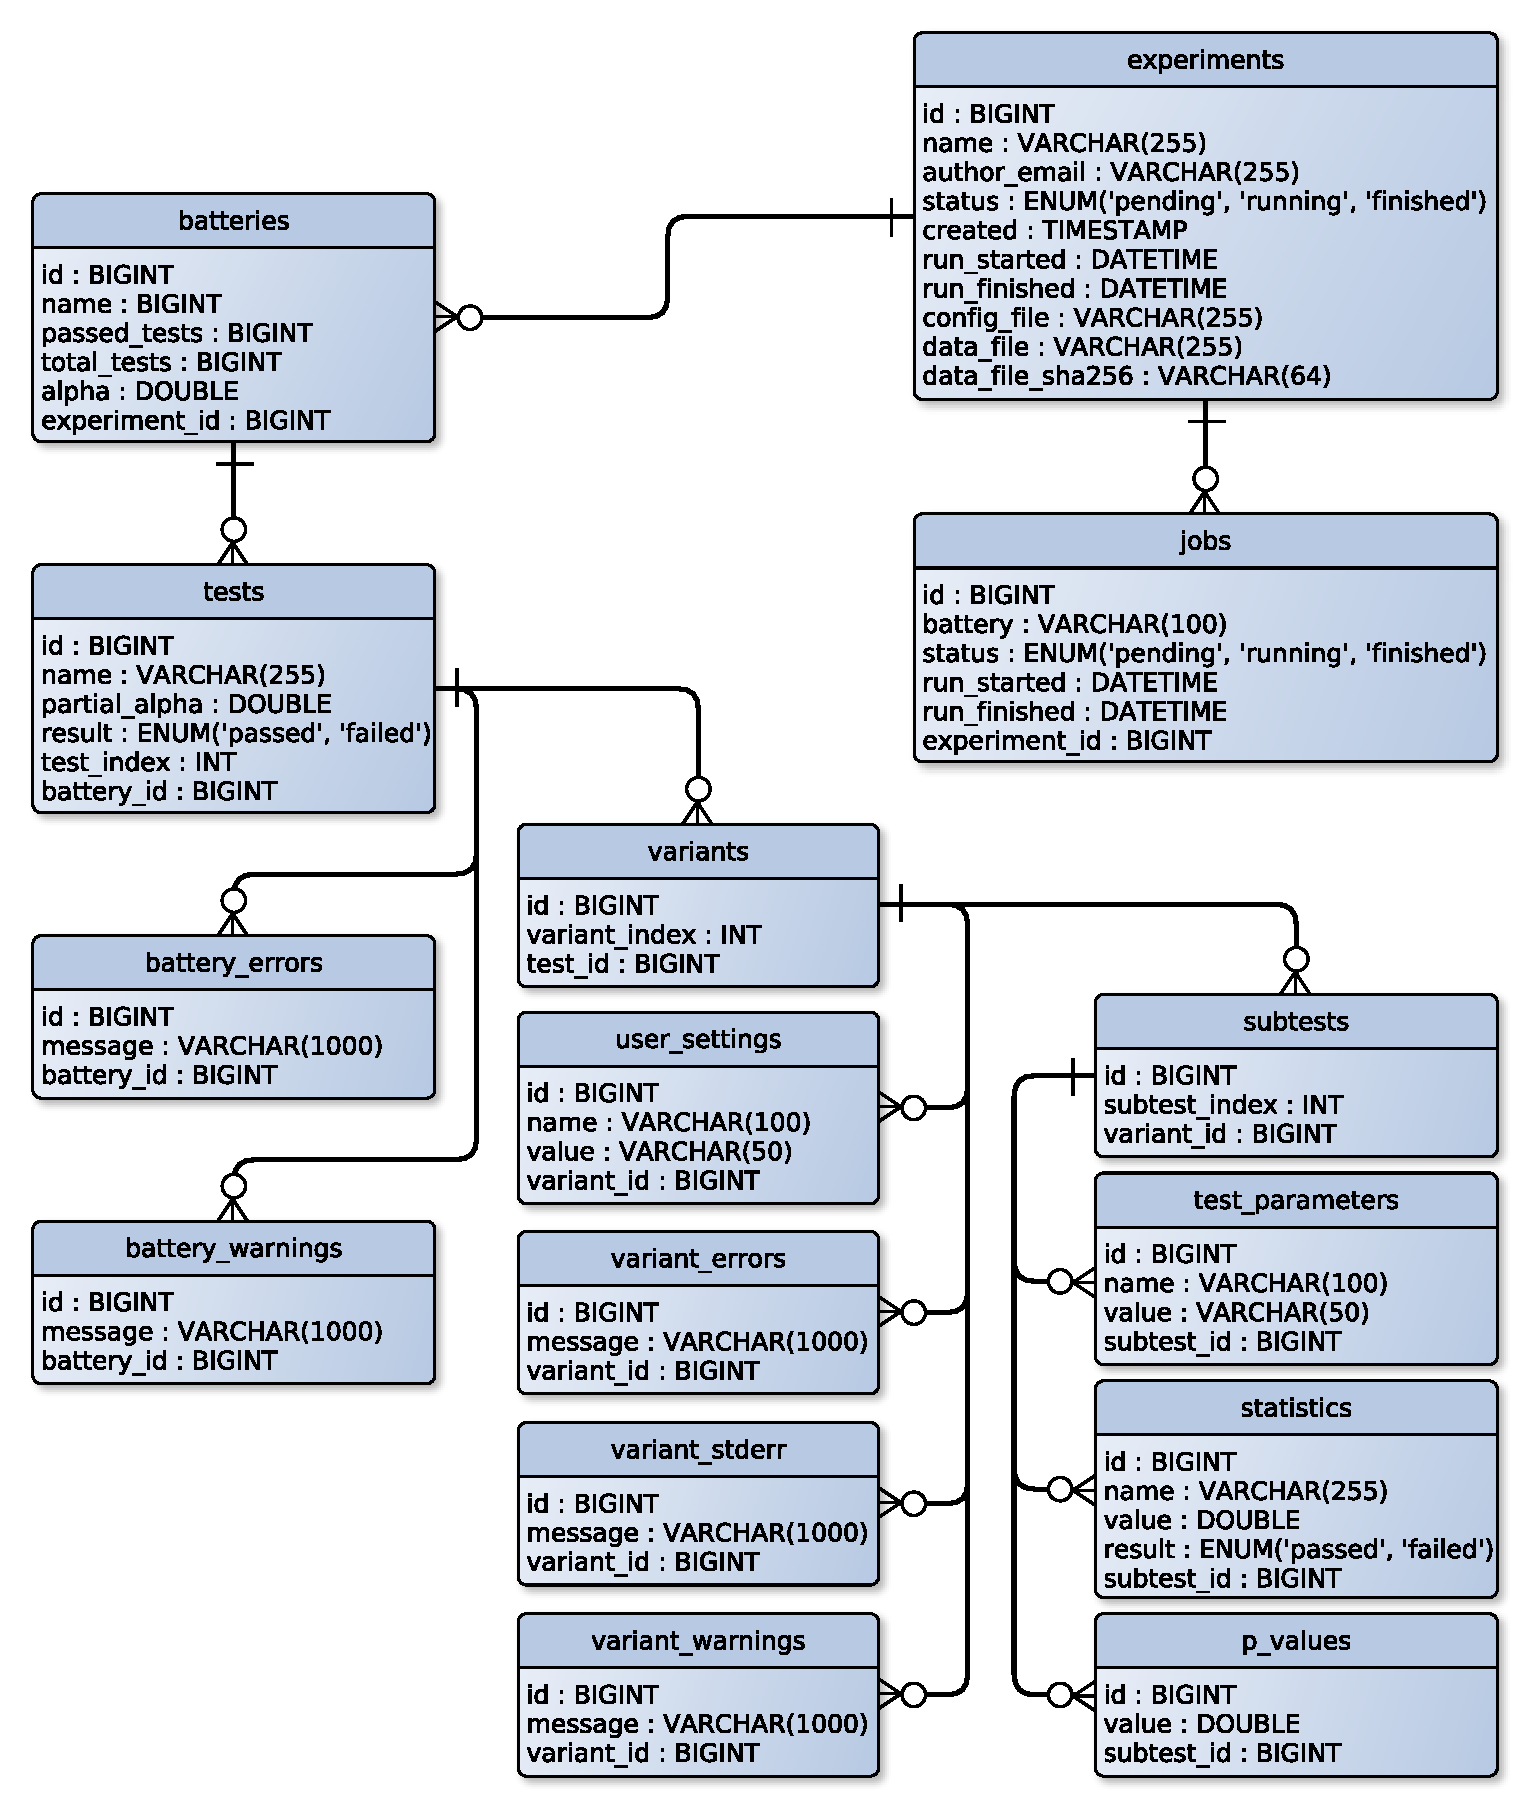
\includegraphics[width=\paperwidth-3.5cm]{figures/database-erd-model.pdf}
\end{nomar}
\caption{ERD Model of the database}
\label{fig:erd_database}
\end{figure}

\begin{description}
\item[\texttt{experiments}] \hfill \\
We treat multiple analyses of single data stream by various batteries as a single experiment. The table stores metadata about the experiment such as name of the analysed file or used configuration file.

\item[\texttt{jobs}] \hfill \\
The table is used for scheduling execution of RTT on remote server. It holds information about the batteries that will be executed and experiment to which they belong. Single job represents a single execution of RTT.

\item[\texttt{batteries}] \hfill \\
Each row represents results of a single execution of RTT. The analysis results are written to this table and its sub-tables by the database storage. The results of multiple RTT executions can be assigned to a single experiment.

\item[\texttt{battery\_errors}, \texttt{battery\_warnings}] \hfill \\
Stores information about errors or warnings that happened during RTT runtime.

\item[\texttt{tests}] \hfill \\
Contains information about the tests that were executed.

\item[\texttt{variants}] \hfill \\
Information about the variants of the tests that were executed.

\item[\texttt{variant\_errors}, \texttt{variant\_stderr}, \texttt{variant\_warnings}] \hfill \\
The errors, warnings and standard error output that were extracted from the outputs of the test variants are stored in the tables.

\item[\texttt{user\_settings}] \hfill \\
Settings that were set by the user in the battery configuration file.

\item[\texttt{subtests}] \hfill \\
Table with the subtests that were executed.

\item[\texttt{test\_parameters}] \hfill \\
Options and parameters that were extracted from the outputs of the subtests.

\item[\texttt{statistics}] \hfill \\
List of all extracted statistics and their results.

\item[\texttt{p\_values}] \hfill \\
List of all extracted p-values.
\end{description}

\section{Remote service}
Randomness Testing Toolkit can be deployed on a single or multiple servers as a service, allowing the users to perform the binary data analysis without the need for the installation of the toolkit and without execution of the tool on their local machine. The statistical testing is, in certain configurations, demanding on computational time and resources. Having the RTT installed on remote machines allows us to scale the resources available for the toolkit and further speed-up the analysis. The user only needs to provide the data for the toolkit and choose (or provide his own) configuration for the batteries. After the testing, the user is notified and can inspect the results.

In the deployment part of the project, we developed an utility project that handles setup and installation of the local interface on single or multiple machines. The deployment project also handles setup of auxiliary scripts and tools that are required for result database and data storage and that will be used by the machines used for statistical testing computation. The database and storage can be deployed on separate machines or on single server that will handle all of the tasks along with the computation of the analysis. 

The interaction of the user with the infrastructure is visualized in Figure~\ref{fig:rtt_ecosystem}. In following section we outline the different purposes of the servers.

\begin{figure}[H]
\begin{nomar}
\centering
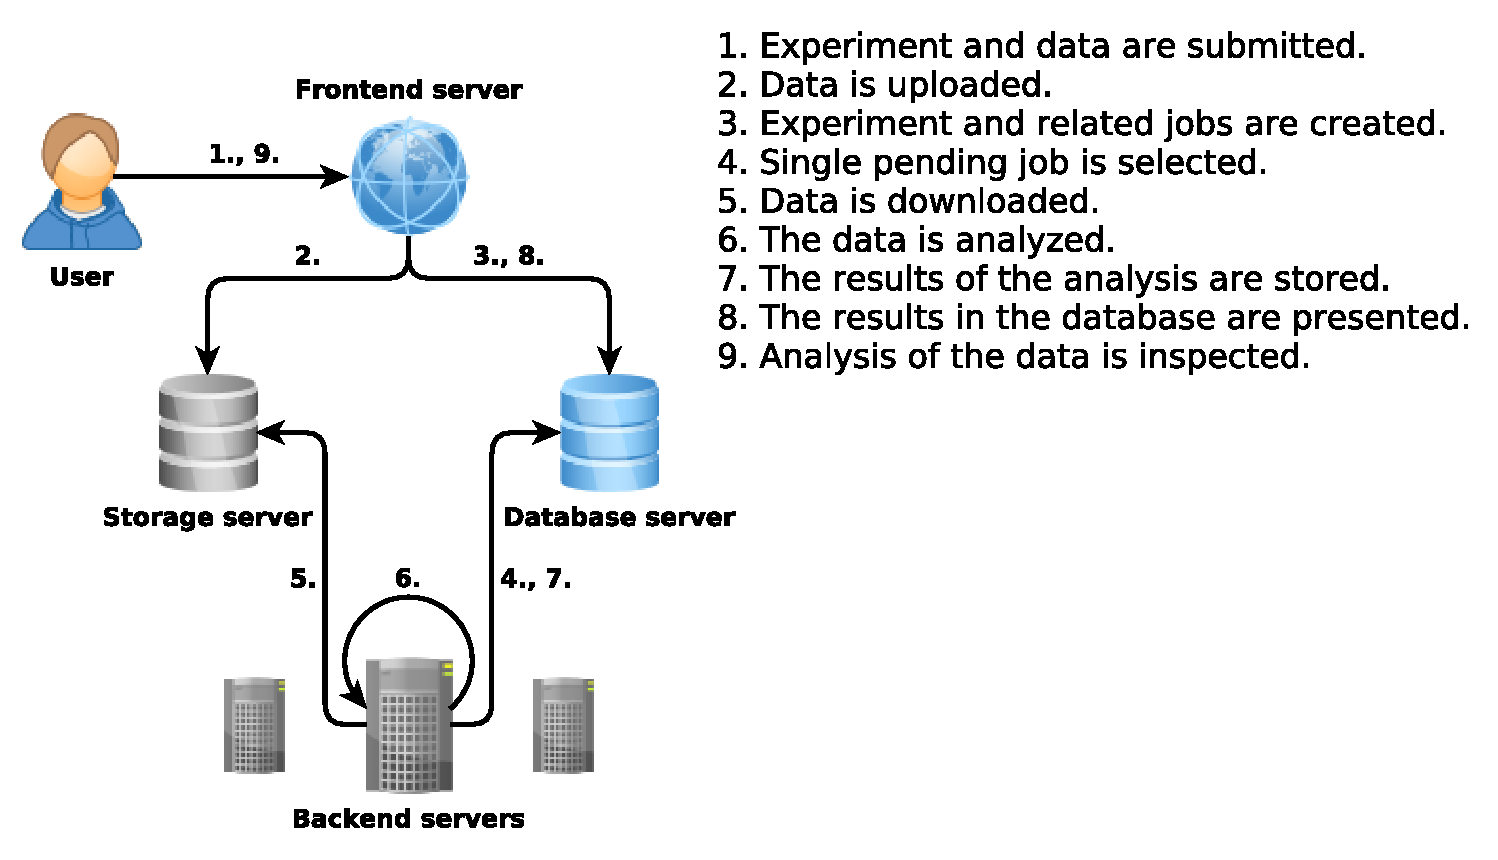
\includegraphics[width=\paperwidth-4cm]{figures/rtt-ecosystem.pdf}
\end{nomar}
\caption{Interaction between user and servers}
\label{fig:rtt_ecosystem}
\end{figure}

\subsection{Database server}
The machine hosting MySQL server with created database for RTT as shown in Figure~\ref{fig:erd_database}. The database is used for storing the results of the analyses as well as the information used for scheduling and distribution of jobs to backend servers.

\subsection{Storage server}
The server hosts a storage space that acts as a temporary deposit for the data that is not yet distributed and analysed on the backend servers. After the distribution and analysis, the data is removed from the machine.

\begin{titlemize}{Scripts on the server}
\item \texttt{clean\_cache.py} -- Script that handles removal of the data files that were already analysed. The script is executed periodically.
\end{titlemize}

\subsection{Backend server}
Single or multiple machines that host the installed toolkit and statistical batteries. The analysis of the data is executed on these machines. If there are multiple backend servers, the computations are scheduled based on the information stored in the database. Prior to the analysis, the data is downloaded from the storage and stored in local cache. After the computation, the results are stored on the database server and the data is deleted.

Both jobs and experiments can be in one of the three states -- \texttt{pending}, \texttt{running} and \texttt{finished}; the descriptions of the states are in Table~\ref{tab:states_jobs_exps}. Scheduling of the computation is based on the state of the experiments and jobs.

\begin{table}[H]
\begin{nomar}
\centering
\begin{tabular}{@{}lp{5cm}p{5cm}@{}} \toprule
\textbf{Status}   & \textbf{Job} & \textbf{Experiment} \\ \midrule
\texttt{pending}  & The job is waiting for execution. & All of the jobs related to the experiment are waiting for execution. \\ 
\texttt{running}  & The job is being executed on backend server. & Some or all related jobs are being executed. \\ 
\texttt{finished} & The jobs execution ended. & The execution of all \newline related jobs ended. \\ \bottomrule
\end{tabular}
\end{nomar}
\caption{States of jobs and experiments}
\label{tab:states_jobs_exps}
\end{table}

\begin{titlemize}{Scripts on the server}
\item \texttt{clean\_cache.py} -- Script that handles removal of the locally cached data files that were already analysed. The script is executed periodically.
\item \texttt{run\_jobs.py} -- Script responsible for choosing the correct computational job, downloading the data from the storage server and the execution of the analysis. Th script is executed periodically. The jobs are picked from the database table \texttt{jobs} with following priority:
\begin{enumerate}
\item Jobs of those experiments whose data was downloaded earlier and the data is present in the local cache of the server.
\item Any jobs of the experiments that are in pending state.
\item Any jobs that are in pending state.
\end{enumerate}
The rules are designed in such a way that a minimal amount of data is transferred over the network. If there are enough distinct pending experiments for all servers then each server will pick single experiment and execute all its jobs and the data of the experiment is transferred only once.
\end{titlemize}

\subsection{Frontend server}
The user interacts only with the frontend server. The machine accepts data and requests for creating an experiment. After the request, the server creates the experiment and the related jobs in the database and uploads the data into the storage. The server also presents the results from the database to the users.

The server can be directly accessed through SSH. The direct access is meant for experienced users that need to analyze big volumes of data. Additionaly, an optional web interface can be deployed on the frontend server. The web interface can be used for interactive browsing of the analysis results as well as for submitting undemanding amount of data and experiments by the users.

The direct access to the server is granted to the user by the system administrator. The RTT users can only access part of the system that is separated from the main system using \texttt{chroot jail} (cit.). The isolated environment contains only the tools and software that is necessary for submitting and processing the experiments. The data for the testing can be uploaded to the server from user's local machine, downloaded from other network location using \texttt{sftp} or generated directly on the server. The data generation is realized with help of the generator tool (cit.) that was developed at CRoCS and is capable of producing outputs of numerous round-reduced cryptographic primitives.

\subsection*{Experiment submission utility}

To create a new experiment, the user has to use utility \texttt{submit\_experiment} that is installed on the server. The utility will transfer the user's data into the storage and will insert new computational jobs into the database. The utility accepts following command-line arguments.

\begin{itemize}
\item \texttt{-h, -{}-help} Prints the usage of the utility.
\item \texttt{-n, -{}-name <name>} Sets the name of the experiment.
\item \texttt{-e, -{}-email <address>} Optional argument. When set, an email with brief results of the analysis will be sent to \texttt{<address>} after the end of the computation.
\item \texttt{-c, -{}-cfg <config-path>} Path to file with configuration of the batteries that will be included in the experiment. Details about configuring the batteries are in Section~\ref{sec:batt_conf}.
\item \texttt{-f, -{}-file <data-path>} Path to file with binary data that will be analysed by the statistical batteries included in the experiment.
\item \texttt{-a, -{}-all\_batteries} Flag argument that will include all of the defined batteries except TestU01 Big Crush in the experiment.
\item \texttt{-{}-nist\_sts} Switch for NIST Statistical Test Suite
\item \texttt{-{}-dieharder} Switch for Dieharder 
\item \texttt{-{}-tu01\_smallcrush} Switch for TestU01 Small Crush
\item \texttt{-{}-tu01\_crush} Switch for TestU01 Crush
\item \texttt{-{}-tu01\_bigcrush} Switch for TestU01 Big Crush
\item \texttt{-{}-tu01\_rabbit} Switch for TestU01 Rabbit
\item \texttt{-{}-tu01\_alphabit} Switch for TestU01 Alphabit
\item \texttt{-{}-tu01\_blockalphabit} Switch for TestU01 Block Alphabit
\end{itemize}

The flags for the batteries switch their inclusion in the experiment. For example, if we use arguments \texttt{"-{}-all\_batteries -{}-dieharder"}, then the batteries included in the experiment will be the batteries added by the \texttt{"-{}-all\_batteries"} flag \textbf{except} the Dieharder battery. However, if we would use only argument \texttt{"-{}-dieharder"}, then Dieharder will be the \textbf{only} battery used is the experiment.

\subsection{Web Interface for RTT}
The web interface is aiming to be useful in the basic use-case, where the user has some binary data in a single file that he wants to analyse. The user will upload the data through the website and will wait for the end of the analysis; the results will be shown on the website after the computation. The web interface is not dependent on or required by the underlying server infrastructure that executes analysis of the data. It was developed only to serve as a user-friendly access point to Randomness Testing Toolkit. For development, we used Django (cit) framework for its ease of use.

In most of the cases, one does not have to create new configuration for the batteries that will be executed during the analysis; a suitable configuration will be chosen for him automatically. Alternatively one can also manually choose the desired configuration or create his own configuration from the scratch according to his preferences.

The limitation of the interface is that the manual creation of large number of experiments would be too time-consuming and error-prone for the user, as the process can't be trivially automated. However the web interface is not intended to be used in such situations; creating the experiments through direct access to the frontend server would be much more viable. 

\subsection*{User roles}
We separate users into three categories in the context of the web interface application. It is worth noting that the user accounts existing in the web interface are independent of the accounts existing on the frontend server. In the following list we summarize the roles and their privileges.

\begin{itemize}
\item \textbf{Anonymous user privileges}
\begin{itemize}
\item Browse results of all previous experiments.
\item Create an experiment if an unique access link was shared with the user.
\end{itemize}
\item \textbf{Authenticated user privileges}
\begin{itemize}
\item Create experiments.
\item Change details and password of the account.
\end{itemize}
\item \textbf{Administrator privileges}
\begin{itemize}
\item Creating new and modifying existing users.
\item Adding administrator privileges to user accounts.
\item Adding or modifying predefined battery configurations.
\item Adding or modifying unique access links to the experiment submission. Each access link has its own expiration date and is unusable after this date.
\end{itemize}
\end{itemize}

\subsection*{Experiment submission}
To create new experiment the user  will have to fill-out following settings in the online form. The screenshot of the form is included in the Appendix~\ref{chap:exp_submit_form}.

\begin{itemize}
\item \textbf{Experiment name} -- Name identifying the experiment, doesn't have to be unique.
\item \textbf{E-Mail} -- Required only when the user is not logged in. After the computation, e-mail will be sent to the address, notifying the user about the results.
\item \textbf{Binary data file} -- Data that will be analysed; uploaded from the user's machine.
\item \textbf{Configuration} -- User can use default battery configuration, choose one of the predefined configurations or upload his own configuration file. The battery configuration files are described in Section~\ref{sec:batt_conf}.
\item \textbf{Battery application} -- Set of switches that defines which batteries will be included in the experiment.
\end{itemize}

\subsection*{Result presentation}
The web interface also presents and assesses the results of the past experiments of all users. Each experiment is listed along with the batteries that were included in it. Battery results are assessed separately; the assessment is based on the proportion of passed and total number of tests included in the battery. We denote this proportion as $x$. Then the probability $P(x)$ of achieving such proportion when testing truly random data is calculated. The calculation process is described in Section TODO. The example of a experiment evalution is shown in Figure~\ref{fig:rtt_assessment}. Based on the probability, the possible assessments are as follows.

\begin{itemize}
\item \textbf{FAIL} ($0 < P(x) < 0.001$) -- The result is deemed as a failure and the source of the data should not be considered as a quality randomness generator.
\item \textbf{Suspect} ($0.001 \leq P(x) < 0.01$) -- The result is considered suspisious. The user should generate more data from the source and test it again. This result is possible to happen by chance even when the tested data is produced by a good source.
\item \textbf{OK} ($0.01 \leq P(x) < 1$) -- The result is evaluated as a good result and the data is considered random.
\end{itemize}

\begin{figure}[H]
\begin{nomar}
\centering
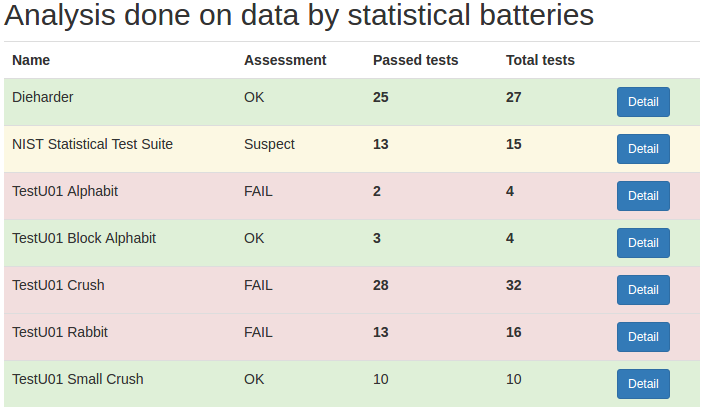
\includegraphics[width=\textwidth]{figures/rtt-assessment.png} 
\end{nomar}
\caption{Experiment evaluation}
\label{fig:rtt_assessment}
\end{figure}

\chapter{Analysing arbitrary binary data with RTT}
\label{chap:crypto_fn_analysis}

In the chapter, we present the results of two distinct experiments and describe the methods and battery configurations used for obtaining the results.

In the first experiment, we analysed large quantities of random data with the statistical batteries implemented in RTT. The motivation for the experiment was that the results of the multiple repeated analyses would provide us with a baseline for our further experiments. Our subsequent experiments would differ from the baseline analysis only in the input data but not in the settings of the respective batteries.

In the second experiment, we analysed outputs of 15 distinct cryptographic algorithms. The specific algorithms were chosen based either on their popularity or their success in cryptographic competitions eSTREAM (cit.) and SHA-3 (cit.); among the selected functions are algorithms such as AES, DES, RC4 or Keccak. We compared the results of the experiment with the results of the analysis in the EACirc framework. The EACirc framework implements an alternative approach to the randomness testing and is developed in CRoCS (cit.).

In our experiments, all statistical tests have significance level $\alpha$ set to 0.01. The tests will reject the null hypothesis $H_0$ based on this significance level.

\section{Battery configurations used in the experiments}
\label{sec:configuration_of_batteries}
In this section, we will present the configurations of the individual batteries that we used in the experiments mentioned above. The settings were kept as close as possible to the default settings of the individual batteries; because of this, the results of the batteries executed through RTT are comparable to the results of the batteries when directly executed. The used RTT battery configuration file is in Appendix~\ref{app:batt_conf_example}.

\subsection{Common settings}
All batteries were provided 8000 MiB\footnote{The exact length of a single file was $8000 \cdot 1024^2 = 8388608000$ bytes.} large data files for the analysis in each execution. The batteries were not required to process the entirety of the data; however rewinding the file and reading more bytes was not permitted to the batteries. We chose the file size as a compromise between the amount of data needed by the separate tests in the batteries and our capabilities to process and store such quantities of data.

\subsection*{NIST Statistical Testing Suite}
The settings of the tests in NIST STS was the same as in default execution of the battery. The tests along with their default settings are listed in Appendix~\ref{app:nist_sts_tests}. In a single run, each test processed 1000 data streams of size 1000000 bits; in total, each test analysed 125 MB of data per execution.

\subsection*{Dieharder}
The test settings of the Dieharder battery follow default settings outlined in Appendix~\ref{app:dieharder_tests} with the single exception of the RGB Lagged Sums test. In default settings, the test would need too much data\footnote{RGB Lagged Sum test with parameter \texttt{n=32} will analyse 13.2 GB of data.} for the analysis. 

The RGB Lagged Sum test is executed in 33 variants with variable parameter \texttt{n=\{0..32\}}. The number of bytes processed by the test variant scales with the parameter \texttt{n} of the variant and the number of times the variant will be repeated (p-samples option) during the battery execution. To lower the amount of the needed bytes, we reduced the number of repetitions for each variant based on its \texttt{n}. The number of repetitions was calculated using the following function.

$$
\text{Rep}(n) = \min\left(100 ; \left\lfloor \frac{ 8000 \cdot 1024^{2} }{ (n + 1) \cdot 4 \cdot 10^{6} } \right\rfloor \right)
$$

\subsection*{TestU01}
We executed the batteries Small Crush and Crush in their default settings. The default settings of the tests in their respective batteries can be found in TestU01 documentation (cit.).

The battery Big Crush is omitted from our analysis because the tests in the battery would need at least 60 GB of data; the amount of data would be infeasible both to generate and store.

The tests in Rabbit, Alphabit and Block Alphabit batteries were executed in their default settings. We limited the tests to 8000 MiB of data by the parameter \texttt{nb}.

The tests in the batteries Alphabit and Block Alphabit have settings that would set them to process only certain parts of each 32-bit block in the data. We did not use these settings; the tests analysed all bits in 32-bit blocks. Additionally, all tests from Block Alphabit are executed in 6 different variants; each test variant analyses differently reordered blocks of 32 bits(cit.).

\section{Baseline experiment}
The aim of this experiment was to observe behaviour and results of the batteries in RTT when analysing truly random data.  We will use the results of this analysis to interpret the results of our further analyses.

We evaluate the battery analysis based on the number of failed tests in the battery. Under the assumption that we have single second-level p-value per single test, the test is considered failed when its p-value is outside of the interval $[\alpha, 1)$; null hypothesis $H_0$ of the test is rejected. The reason why we excluded one from the non-rejecting interval is explained in Section~\ref{sec:preventive_measures_rtt}.

When analysing a truly random data repeatedly with a statistical test, we will observe that the resulting p-values are uniformly distributed on the interval $[0,1]$. The uniformity is caused by the fact that we can't predict the output of a TRNG and each possible output is observed with equal probability. Therefore, we also can't predict the result of the analysis with a statistical test. Since the p-values are uniformly distributed, they will fall outside of the interval $[\alpha, 1)$ with probability equal to $\alpha$; test's $H_0$ will be rejected with probability $\alpha$. When the null hypothesis of a test is rejected, we assess the test as failed.

When we are evaluating a battery analysis based on a count of failed tests, we must know how many tests we expect to fail when $H_0$ holds true. We can calculate the expected value like so. Let $n$ be the number of tests in a battery. Then we have $n$ independent experiments that will result in either yes (failure of the test) with probability $\alpha$ or no (success of the test) with probability $1-\alpha$. This situation can be modeled by using binomial distribution (cit.) $\text{Bin}(n, \alpha)$. Let $F_{Exp}$ be a random discrete variable expressing the count of failed tests in a battery with expected distribution $\text{Bin}(n, \alpha)$. From the definition of the binomial distribution, the expected value of a random variable is $E(F_{Exp}) = n\alpha$. Therefore, should a battery finish with $n\alpha$ failed tests we still can't reject $H_0$ for the whole battery; we will treat the analysed data as random.

However, the expected number of failures is not necessarily exact, as the calculation described above treats tests as independent trials. Separate tests in a battery are not required nor proved to be independent, which can lead to differing distributions of empirical and theoretical random variables representing the counts of failed tests in the batteries.

To observe the empirical distribution of the number of failed tests $F_{Obs}$, we inspected the number of failures of the individual batteries during the analysis of truly random data. In total, approximately eight terabytes of random data were downloaded from QRNG service provided by Humboldt-Universitaet zu Berlin (cit.). The data were split into 1000 blocks each of size 8000 GiB. All seven batteries included in this experiment analysed each block of data once. The sample size of 1000 trials is enough for us to compare the distributions of the two random variables $F_{Exp}$ and $F_{Obs}$.

We inspected the counts of failures of individual batteries in following two scenarios.

\begin{description}
\item[Original second-level p-values failures] \hfill \\
In this scenario, we assumed that all second-level p-values produced by a specific battery are independent. Therefore, we treated all statistics calculated by the battery as separate tests. For example, if we execute some test in two variants, each of those variants has two subtests, and each subtest will calculate two statistics, in total we will get $2^3=8$ second-level p-values; we consider these eight p-values as the results of eight independent tests each of whose calculated a single p-value. 

\item[Corrected p-values failures] \hfill \\
With this second scenario, we tried to mitigate the effect of dependent p-values in our set by grouping them together. We grouped the p-values that are most likely dependent; we assumed that the p-values that are most likely inter-connected are those that are produced by a single statistical test. Therefore, all p-values belonging to a single test were reduced to only one p-value, leaving us with a single result per distinct test in a statistical battery. For example, should a single test produce eight p-values, for this test we will only have information whether the test was a failure or not. For the grouping of the p-values, we used Šidák's correction (cit.), and we show the process in Definition~\ref{def:sidak}.

\begin{definition}
\label{def:sidak}
For a multiset of $n$ grouped p-values $P = \{p_1,..,p_n\}$ with significance level $\alpha$ and null hypothesis $H_0$ we will calculate the corrected significance level $\alpha_0 = 1 - (1 - \alpha)^{\frac{1}{n}}$. If $\exists p \in P : (p < \alpha_0) \vee (p = 1) $, then $H_0$ is rejected for $\forall p \in P$ and the whole group result is treated as a failure.
\end{definition}

\end{description}

To compare the feasibility of the two scenarios, we needed to compare both of the observed distributions to their respective expected distributions and see how they perform. We consider the approach more feasible when it is less differing from its expected distribution; the battery results are easier to interpret when they are closer to the theoretical expectations. In the rest of the section, we describe the comparison process.

\begin{definition}
\label{def:freq}
Let $X = \{x_1, .. ,x_n\}$ be a multiset of $n$ elements. Then we define frequency variable $f_{e}^{X}$ as the frequency of element $e$ in multiset $X$. If $\nexists e, x \in X : e = x$, then $f_{e}^{X} = 0$.
\end{definition}

During this experiment each battery was executed 1000 times; for each battery we had $s = 1000$ samples of a discrete random variable $F_{Obs}$, expressing the count of failed tests in that battery. Random variable $F_{Exp}$ expresses the theoretical expected count of failures in a battery with $n$ test and the significance level $\alpha$. Variable $F_{Exp}$ follows binomial distribution $\text{Bin}(n, \alpha)$. The probability of observing $x$ test failures (written as $F_{Exp} = x$) in $\text{Bin}(n, \alpha)$ is defined with probability mass function of binomial distribution (Equation~\ref{eq:bin_pmf}).

\begin{equation}
\label{eq:bin_pmf}
P(F_{Exp} = x) = \binom nx \alpha^x (1-\alpha)^{n-x} 
\end{equation}

Let $X = \{x_1,..,x_s\}$ be a multiset of the samples of $F_{Obs}$ and $D = \{d_1,..,d_k\}$ set of all $k$ distinct values in $X$. Then $f_{d}^{X}, d \in D$ (see Definition~\ref{def:freq}) represents a random variable expressing the frequency of a failure count within a multiset $X$. The random variable $f_{d}^{X}$ is expected to follow binomial distribution $\text{Bin}(s, p)$ where $s$ is the number of samples and $p$ is the probability of observing $d$ failures ($P(F_{Exp} = d)$, Equation~\ref{eq:bin_pmf}). The expected value of the random variable $f_{d}^{X}$ is defined using expected value of binomial distribution (Equation~\ref{eq:exp_freq}).

\begin{equation}
\label{eq:exp_freq}
E\left(f_{d}^{X}\right) = s P(F_{Exp} = d)
\end{equation}

Now that we have both the observed frequency $f_{d}^{X}$ and its expected value $E\left(f_{d}^{X}\right)$ for $d \in D$, we can assess their closeness. For this assessment, we used Pearson's chi-squared test ($\chi^2$) that evaluates whether any observed difference between two data sets happened by a chance (cit.). We calculated Pearson's cumulative test statistic $\chi^2$ for each pair of expected and observed frequencies as shown in Equation~\ref{eq:chi_square_stat}.

\begin{equation}
\label{eq:chi_square_stat}
\chi^2 = \sum\limits_{i=1}^{k} \frac{  \left(f_{d_i}^{X} - E \left(f_{d_i}^{X}\right) \right)^2 }{E \left(f_{d_i}^{X}\right)}
\end{equation}

Due to the limitation of Pearson's $\chi^2$ test stating that the expected value must be at least 5, the samples that didn't satisfy this condition were summed together and treated as a single sample. We then calculated p-value using $\chi^2$ distribution (cit.). The p-value calculation is based on the number of the degrees of freedom that is equal to $k-1$ and the value of $\chi^2$ statistic. The p-value of the $\chi^2$ test statistic can be calculated as $1 - \text{CDF}(df, \chi^2)$, where CDF is the cumulative distribution function of the $\chi^2$ distribution, df are the degrees of freedom and $\chi^2$ is the value of the $\chi^2$ test statistic.

The resulting p-value is an indicator of how close are the two tested datasets. The p-value expresses the probability that any difference between the two measured sets happened by chance. Therefore, when we are comparing the feasibility of the two failure counting scenarios (original versus corrected results) the more feasible one will have higher p-value than the other; our point was to find out which one of our approaches followed our theoretical expectations more closely.

\begin{figure}[H]
\begin{nomar}
\centering

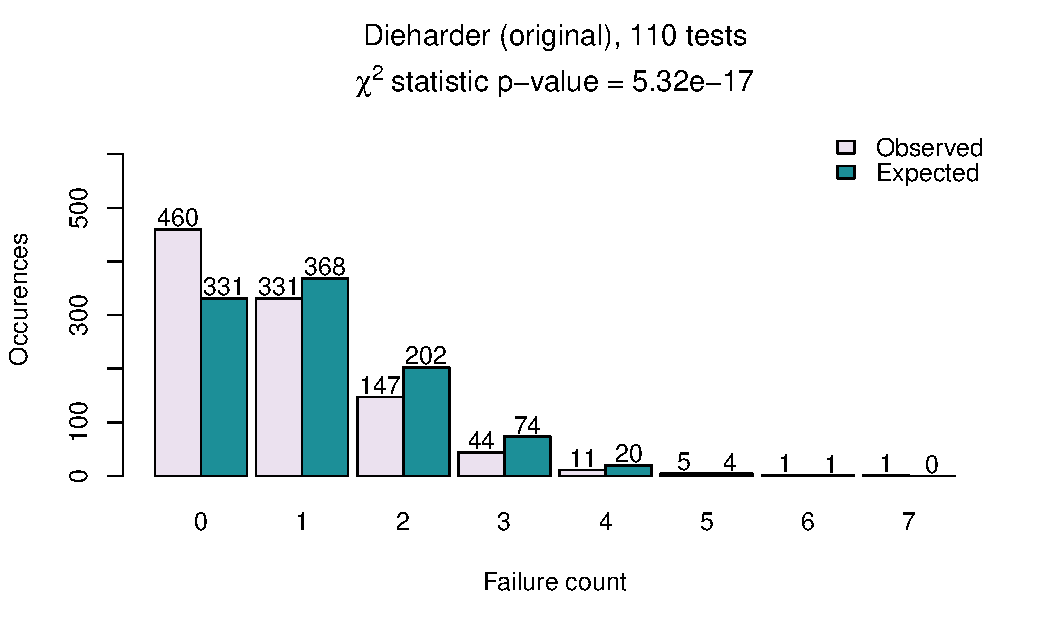
\includegraphics[width=.42\paperwidth]{figures/dieharder-orig.pdf} 
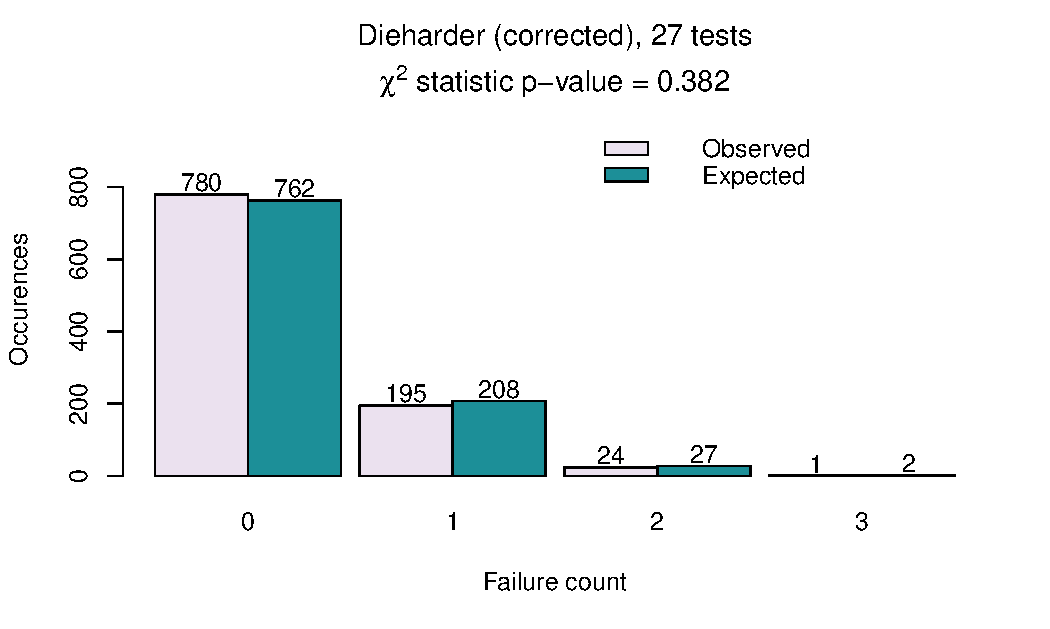
\includegraphics[width=.42\paperwidth]{figures/dieharder-corr.pdf} 

\end{nomar}
\caption{Test failure frequency distributions in Dieharder battery}
\label{fig:corr_vs_orig_hist}
\end{figure}

In Figure~\ref{fig:corr_vs_orig_hist} we can see both the original and the corrected failure frequencies along with their expected distributions. As the $\chi^2$ statistic p-value suggest, in the corrected version of failure counting, the observed failure frequency is much closer to the expected distribution than in the original version.

\begin{table}[H]
\begin{nomar}
\centering

\begin{tabular}{@{}lrrrrr@{}} \toprule
& \multicolumn{2}{c}{\textbf{Original} $F_{Obs}$} & \multicolumn{2}{c}{\textbf{Corrected} $F_{Obs}$} &  \\ \cmidrule(lr){2-3} \cmidrule(lr){4-5}
\textbf{Name} & $\chi^2$ & $\max(F_{Obs})$& $\chi^2$ & $\max(F_{Obs})$ & \textbf{Acc. bound} \\ \midrule
Dieharder      & $5.32 \cdot 10^{-17}$    &  7/110 & \gr$0.38$                & 3/27 & 3/27 \\
NIST STS       & \gr$2.17 \cdot 10^{-2}$  &  7/188 & $4.44 \cdot 10^{-7}$     & 3/15 & 2/15 \\
Small Crush    & $0.71$                   &   3/15 & \gr$0.95$                & 2/10 & 2/10 \\
Crush          & $3.36 \cdot 10^{-11}$    &  8/186 & \gr$3.31 \cdot 10^{-3}$  & 3/32 & 3/32 \\
Rabbit         & \gr$2.02 \cdot 10^{-5}$  &   6/58 & $1.45 \cdot 10^{-23}$    & 2/16 & 2/16 \\
Alphabit       & $2.14 \cdot 10^{-8}$     &   8/33 & \gr$2.8 \cdot 10^{-7}$   & 2/4  & 1/4 \\
Block Alphabit & $1.87 \cdot 10^{-68}$    & 14/198 & \gr$5.15 \cdot 10^{-47}$ & 3/4  & 1/4 \\ \bottomrule
\end{tabular}

\end{nomar}
\caption{Summary of test failure distributions and acceptance bound of the batteries}
\label{tab:baseline_summary}
\end{table}

In Table~\ref{tab:baseline_summary} we present comparison of the $\chi^2$ statistic p-values between the original and the corrected results. We can see, that in general, the corrected results are closer to their expected distributions. Only in two cases (NIST STS and Rabbit), the corrected results perform worse while in the remaining batteries they offer a significant improvement. We also present the acceptance bounds for the batteries. The acceptance bound represents the maximum number of failed tests in a battery, while not rejecting the null hypothesis. Should the number of failures exceed the acceptance bound, we will reject $H_0$; the tested data failed to pass the battery.

However, even with the improved result interpretation, some failure frequencies are still too distant from their theoretical distributions. For this reason, we decided to increase the acceptance bounds. We set the acceptance bounds in such a way that the probability of Type I error is not higher than 0.001.

The presented bounds are used for result interpretation of the subsequent experiments. If the number of failed tests will be higher than the bound, the data did not pass the battery analysis.

\section{Analysis of well-known cryptographic algorithms}
In this experiment, we focused on the analysis of well-known and used cryptographic primitives. The 15 algorithms were chosen based on their popularity and success in cryptographic competitions eSTREAM (cit.) and SHA-3 (cit.).

Our motivation for this experiment was to find out how big are the security margins on conventional algorithms. Most of the tested algorithms could be reduced in the number of their rounds. We wanted to see how much could we reduce the rounds until we would start detecting the biases in the data.

The outputs of the functions were generated using the generator developed in CRoCS (cit.). The plaintext of the functions was a binary counter; the key was randomly generated, and initialization vector was set to zeroes. Not all functions needed the key and IV. 

For each particular round and function combination, we generated 8000 MiB large data file. In total,  we analysed 72 distinct combinations of functions and rounds. The configurations of the batteries were the same as described in Section~\ref{sec:configuration_of_batteries}. 

The results of this experiment were also compared to the results produced by the EACirc framework (cit.). The results of the analysis of the data with EACirc are part of Karel Kubíček's diploma thesis (cit.).

\subsection{Results of the analysis}
The results of the analysis are shown in Table~\ref{tab:crypto_alg_analysis}. We included only the combinations of algorithms and rounds in which the data failed to pass either EACirc or any battery in RTT. The marked cells in the table indicate failure of the tool. 

\begin{table}[H]
\begin{nomar}
\centering

\scalebox{0.85}{
\begin{tabular}{@{}lrrrrrrrrrrrr@{}} \toprule
\textbf{\large Algorithm} & 
\multicolumn{1}{R{3.2cm}}{\textbf{Round}} &
\multicolumn{1}{R{3.2cm}}{\textbf{Total rounds}} &
\multicolumn{1}{R{3.2cm}}{\textbf{NIST STS} \\ \footnotesize (x/15)} &
\multicolumn{1}{R{3.2cm}}{\textbf{Dieharder} \\ \footnotesize (x/27)} &
\multicolumn{1}{R{3.2cm}}{\textbf{Small Crush} \\ \footnotesize (x/10)} &
\multicolumn{1}{R{3.2cm}}{\textbf{Crush} \\ \footnotesize (x/32)} &
\multicolumn{1}{R{3.2cm}}{\textbf{Rabbit} \\ \footnotesize (x/16)} &
\multicolumn{1}{R{3.2cm}}{\textbf{Alphabit} \\ \footnotesize (x/4)} &
\multicolumn{1}{R{3.2cm}}{\textbf{Block Alphabit} \\ \footnotesize (x/4)} &
\multicolumn{1}{R{3.2cm}}{\textbf{EACirc} \\ \footnotesize (proportion)} &
\multicolumn{1}{R{3.2cm}}{\textbf{Security margin} \\ \footnotesize (rounds)} &
\multicolumn{1}{R{3.2cm}}{\textbf{Security margin} \\ \footnotesize (proportion)} \\ \midrule
% nist diehard small crush crush rabbit alphabit blockalphabit eacirc
AES        &  3 &  10 &  \rd8 & \rd15 &  \rd5 & \rd20 &  \rd5 &  \rd2 &  \rd4 & \rd0.182 & 7 & \ctwo 0.70 \\ \midrule
BLAKE      &  1 &  16 & \rd11 & \rd11 &  \rd5 & \rd18 & \rd5 &  \rd2 &  \rd3 & \rd0.107 & 15 & \cone 0.93 \\ \midrule
Grai$\text{n}^{\ast}$      &  2 &  13 & \rd14 & \rd27 & \rd9/9&\rd31/31& \rd15 &  \rd4 &  \rd4 & \rd1.000 & 7 & \cthree 0.53 \\
           &  6 &     &  1 &  0 &  0 &  3 &  1 &  0 &  0 & 0.017 &  & \\ \midrule
Gr\o stl   &  2 &  14 & \rd12 & \rd23 &  \rd9 & \rd27 &  \rd9 &  \rd3 &  \rd3 & \rd1.000 & 12 & \cone 0.85 \\ \midrule
JH         &  6 &  42 &\rd12/13& \rd27 & \rd10 &\rd30/31& \rd15 &  \rd4 &  \rd4 & \rd1.000 & 36 & \cone 0.85 \\ \midrule
Keccak     &  2 &  24 & \rd14 & \rd27 & \rd10 & \rd31 & \rd15 &  \rd4 &  \rd4 & \rd1.000 & 21 & \cone 0.87 \\
           &  3 &     &  0 &  1 &  1 & \rd11 &  \rd4 &  0 &  \rd3 & 0.017 &  & \\ \midrule
MD$\text{6}^{\ast}$         &  8 & 104 &  \rd9 & \rd19 &  \rd5 & \rd16 &  \rd8 &  \rd2 &  \rd3 & \rd0.748 & 94 & \cone 0.90 \\
           & 10 &     &  0 &  0 &  0 &  2 &  \rd3 &  0 &  0 & 0.010 &  & \\ \midrule
Rabbi$\text{t}^{\ast}$      &  0 &   4 &  1 &  1 &  0 &  \rd4 &  \rd3 &  1 &  1 & 0.017 & 0 & \cfour 0 \\
           &  4 &     &  0 &  0 &  0 &  3 &  \rd3 &  1 &  1 & 0.009    &  & \\ \midrule
Salsa20    &  2 &  20 & \rd12 & \rd26 &  \rd8 & \rd28 & \rd11 &  \rd3 &  \rd3 & \rd1.000 & 18 & \cone 0.90 \\ \midrule
Single DES &  4 &  16 &  \rd7 & \rd22 &  \rd7 & \rd26 & \rd11 &  \rd4 &  \rd4 & \rd0.193 & 11 & \ctwo 0.68 \\
           &  5 &     &  1 &  \rd6 &  1 & \rd18 &  \rd5 &  \rd2 &  \rd3 & 0.010 &  & \\ \midrule
Skein      &  3 &  72 & \rd12 & \rd27 & \rd10 & \rd30 & \rd13 &  \rd3 &  \rd4 & \rd1.000 & 68 & \cone 0.94 \\
           &  4 &     &  0 &  0 &  0 & \rd10 &  \rd4 &  1 &  \rd3 & 0.014 &  & \\ \midrule
SOSEMANUK  &  4 &  25 & \rd13/13 &\rd27& \rd10 &\rd31/31& \rd16 & \rd4  &  \rd4 & \rd1.000 & 21 & \cone 0.84 \\ \midrule
TEA        &  4 &  32 & \rd8 & \rd19 &  \rd6 & \rd15 & \rd4 &  \rd2 &  \rd3 & \rd0.444 & 27 & \cone 0.84 \\
           &  5 &     &  0 &  3 &  2 &  \rd4 &  1 &  0 &  \rd3 & 0.012 &  & \\ \midrule
Triple DES &  2 &  16 & 1\rd2 & \rd26 &  \rd9 & \rd31 & \rd15 &  \rd3 &  \rd4 & \rd1.000 & 13 & \cone 0.81 \\
           &  3 &     &  1 &  \rd4 &  1 &  \rd4 &  0 &  1 &  1 & 0.017 &  & \\ \midrule
RC$\text{4}^{\ast}$  (roundless) & -- & -- & 0 & 0 & 0 & 3 & 0 & 0 & 0 & 0.009 & -- & \cfour 0 \\
\bottomrule
\end{tabular}
}

\end{nomar}
\caption{Results of the analysis of cryptographic algorithms}
\label{tab:crypto_alg_analysis}
\end{table}

The values in the battery columns express the number of failed tests in a specific battery. Each battery has defined the total number of tests in the header. In some cases, not all tests in the battery could be executed; in these cases, we specify the number of performed tests in the cell. 

The values in EACirc column display the proportion of EACirc executions that rejected the null hypothesis for the tested data. We do not consider the data random when the value of the proportion is higher than 0.2.

We also provide security margins of the analysed algorithms. The security margins are based on the highest round in which the algorithm failed to pass any battery and on the default total number of rounds in the algorithm.

Some algorithms in the table are marked by an asterisk. In highest shown rounds, these algorithms did pass most of the batteries; however, after closer inspection, we discovered some patterns in the results. These findings are summarized in Section~\ref{sec:notable_results}.

The discovered patterns in the results were consistent failures of certain tests when analysing algorithm with fixed number of rounds. We consider a test as consistently failing when we create multiple datasets of the same algorithm and round and the test will fail in all analyses of the datasets. The generation of the datasets can vary in the used keys or plaintexts.

For each suspicious algorithm with fixed number of rounds, we generated additional 16000 MiB of data. The additional data showed the same patterns in the results as in the original analysis, hinting the presence of a particular bias produced by the algorithm.


\subsection{Notable observations}
\label{sec:notable_results}
In this section, we list our observations based on the above-presented results, according to their importance.

\begin{description}
\item[Biased output of the Rabbit cipher] \hfill \\
Rabbit cipher is one of the winners in the eSTREAM competition in the software section. The algorithm has a total of 4 rounds. In all of its configurations, Rabbit will consistently fail tests \texttt{sstring\_HammingIndep} and \texttt{sstring\_PeriodsInStrings} in batteries Crush, Rabbit, Alphabit and Block Alphabit. 

The tests are aiming to discover dependencies between separate bits in the data stream. One interesting detail is that the tests in Block Alphabit will fail if and only the bits in the stream are not previously re-ordered by the battery. This fact led us to believe that there indeed is some dependency between bits in the output.

Biases in the output of the Rabbit cipher were previously published in papers \textit{On a bias of Rabbit}(cit.) and \textit{Cryptanalysis of Rabbit} (cit.). The authors of the latter paper claimed to be able to construct distinguisher for the cipher with the complexity of $2^{158}$.

\item[Biased output of the RC4 cipher] \hfill \\
RC4 is a popular stream cipher widely used in WEP and TLS up until version 1.3. Various attacks on RC4 were published, and in 2015 it was prohibited for use in TLS by RFC 7465 (cit.). In its full version, the RC4 cipher will consistently fail tests \texttt{sknuth\_SimpPoker} and \texttt{sknuth\_Gap} in the Crush battery.

There are multiple known biases and distinguishing attacks on RC4; notable publications are \textit{A Practical Attack on Broadcast RC4} (cit.), \textit{Analysis of Non-fortuitous Predictive States of the RC4 Keystream Generator} (cit.) and \textit{Statistical Analysis of the Alleged RC4 Keystream Generator} (cit.). Any of these biases can be causing the failure of the statistical tests.

\item[Security margins with respect to the statistical analysis] \hfill \\
The majority of the analysed algorithms has the security margin higher than 0.8. This means that even if we would drastically increase our computational capability and performance of the state-of-the-art statistical tools we still wouldn't be able to detect biases in most of the function outputs. 

The margins are significantly lower only for functions with particular biases detected, namely Rabbit, RC4 and Grain.

\item[Strength of the batteries and EACirc] \hfill \\
All of the batteries implemented in RTT perform better or equally well than EACirc. The shortcomings of EACirc can be caused by the fact that the framework analyses only 100 MB of data per execution and also finishes its execution more quickly. Therefore we have a trade-off between the needed time and resources and strength of the tool. In many situations we aren't able to retrieve 8000 MiB (e.g. slow hardware generators in smartcards); in these cases, the usage of EACirc for bias detection can be viable.

The batteries themselves have differing strength. While batteries NIST STS and Small Crush have more or less same bias detection capabilities as EACirc, the remaining batteries perform better and can detect even subtle biases. The remaining batteries are listed here, along with the number of times they detected a bias when other batteries failed to do so: Alphabit (2 times), Dieharder (3 times), Block Alphabit (5 times), Rabbit (6 times), Crush (8 times).

\item[Biased output of round reduced Grain function] \hfill \\
The Grain algorithm is on of the winners of the eSTREAM competition in the hardware section. In 3, 4, 5 and 6 rounds out of 13, the test will consistently fail tests \texttt{smarsa\_MatrixRank} and \texttt{scomp\_LinearComp} in batteries Crush and Rabbit.  Bias in 6 rounds does not break the security of the cipher, but due to its existence, the security margin is significantly lower (around 0.5) than in other well-known functions. 

\item[Biased output of round reduced MD6 hash function] \hfill \\
The MD6 hash function was a competitor in the SHA-3 competition but did not advance to the second round of the competition. In 9 and 10 rounds out of 94, the algorithm will consistently fail tests \texttt{smarsa\_MartixRank} and \texttt{sspectral\_Fourier3} in batteries Crush and Rabbit. While this hints us with the presence of a specific bias in the function output it does not break the security of the function; in further rounds, we can no longer detect any bias, and the output appears as truly random.

\end{description}
























































































































































\chapter{Analysis of DIEHARDER results on quantum random data}
\begin{itemize}
\item Statistical intro, uniformity, first vs. second level p-value, etc...
\item Two experiments - continuous p-values, blocks of 2nd level
\item Results - non-uniform, where it will begin to show on 2nd level results
\end{itemize}

\chapter{Conclusions}
\begin{itemize}
\item Developed user-friendly tool for easy analysis of arbitrary binary data - Randomness Testing Toolkit
\item Interpretation of results
\item Comparison of batteries with EACirc, polynomials
\item Defects in Dieharder, their relevance, etc...
\item Future work, same analysis on TestU01, dependence between tests(?), continuous development of RTT, call for flawless statistical battery ( :) )
\end{itemize}

\appendix

\printbibliography

\chapter{NIST STS Tests}
\label{app:nist_sts_tests}

\begin{titlemize}{Common parameters of all tests}
\item \textbf{Stream size} -- 1000000
\item \textbf{Stream count} -- 1000
\end{titlemize}

\begin{nomar}
\centering
\begin{tabular}{@{}rlrr@{}} \toprule
\textbf{ID} & \textbf{Test name} & \textbf{Block size} & \textbf{Subtests} \\ \midrule
1  & Frequency (Monobit)                           & --  & 1 \\
2  & Frequency within a Block                      & 128 & 1 \\
3  & Cumulative Sums (Cusums)	                   & --  & 2 \\
4  & Runs                                          & --  & 1 \\
5  & Longest Run of Ones in a Block                & --  & 1 \\
6  & Random Binary Matrix Rank                     & --  & 1 \\
7  & Discrete Fourier Transform (Spectral)         & --  & 1 \\
8  & Non-overlapping (Aperiodic) Template Matching & 9   & 148 \\
9  & Overlapping (Periodic) Template Matching      & 9   & 1 \\
10 & Maurer's “Universal Statistical” 	           & --  & 1 \\
11 & Approximate Entropy 	                       & 10  & 1 \\
12 & Random Excursions 	                           & --  & 8 \\
13 & Random Excursions Variant	                   & --  & 18 \\
14 & Serial                                        & 16  & 2 \\
15 & Linear Complexity	                           & 500 & 1 \\ \bottomrule
\end{tabular}
\end{nomar}

\chapter{Dieharder Tests}
\label{app:dieharder_tests}
\textbf{Note:} Tests labeled as not used are excluded from our experiments; they are flagged as suspicious or not working in Dieharder documentation. Tests with plus sign next to the stream size will process variable amount of data on each run. The value is only orientational.

\begin{nomar}
\centering

\scalebox{0.9}{
\begin{tabular}{@{}rlrrl@{}} \toprule
\textbf{ID} & \textbf{Test name} & \textbf{Stream size (byte)} & \textbf{P-samples} & \textbf{Arguments} \\ \midrule
\multicolumn{5}{c}{\textbf{Diehard tests}} \\ \midrule
0   & Birthdays                    &    153 600 & 100 & -- \\
1   & OPERM5                       &  4 000 020 & 100 & -- \\
2   & 32$\times$32 Binary Rank     &  5 120 000 & 100 & -- \\
3   & 6$\times$8 Binary Rank       &  2 400 000 & 100 & -- \\
4   & Bitstream                    &  1 048 584 & 100 & -- \\
5   & OPSO \textbf{(Not used)}     &         -- & --  & -- \\
6   & OQSO \textbf{(Not used)}     &         -- & --  & -- \\
7   & DNA \textbf{(Not used)}      &         -- & --  & -- \\
8   & Count the 1s (stream)        &    256 004 & 100 & -- \\
9   & Count the 1s (byte)          &  5 120 000 & 100 & -- \\
10  & Parking Lot                  &     96 000 & 100 & -- \\
11  & Minimum Distance (2D Circle) &     64 000 & 100 & -- \\
12  & Minimum Distance (3D Sphere) &     48 000 & 100 & -- \\
13  & Squeeze 					   & 10 000 000+& 100 & -- \\
14  & Sums \textbf{(Not used)}     &         -- & --  & -- \\
15  & Runs                         &    400 000 & 100 & -- \\
16  & Craps                        & 10 000 000+& 100 & -- \\ \midrule
\multicolumn{5}{c}{\textbf{Marsaglia and Tsang tests}} \\ \midrule 
17  & GCD & 80 000 000 & 100 & -- \\ \midrule
\multicolumn{5}{c}{\textbf{STS tests}} \\ \midrule
100 & Monobit              & 400 000 & 100 & -- \\
101 & Runs                 & 400 000 & 100 & -- \\
102 & Serial (Generalized) & 400 000 & 100 & -- \\ \midrule
\multicolumn{5}{c}{\textbf{RGB tests}} \\ \midrule
200 & Bit Distribution             & n$\times$800 000 + 4 & 100 & \texttt{-n \{1..12\}} \\
201 & Generalized Minimum Distance & n$\times$40 000 & 100 & \texttt{-t 10000 -n \{2..5\}} \\
202 & Permutations                 & n$\times$400 000 & 100 & \texttt{-n \{2..5\}} \\
203 & Lagged Sum                   & (n+1)$\times$4 000 000 & 100 & \texttt{-n \{0..32\}} \\
204 & Kolmogorov-Smirnov           & 40 000 & 1000 & -- \\ \midrule
\multicolumn{5}{c}{\textbf{DAB tests}} \\ \midrule
205 & Byte Distribution & 614 400 000 & 1 & -- \\
206 & DCT               &  51 200 000 & 1 & -- \\
207 & Fill Tree         & 500 000 000+& 1 & -- \\
208 & Fill Tree 2       & 200 000 000+& 1 & -- \\
209 & Monobit 2         & 260 000 000 & 1 & -- \\ \bottomrule
\end{tabular}
}
\end{nomar}

\chapter{Overview of options in toolkit settings}
\label{app:toolkit_settings_detail}

The tags that are listed in the top-level description must contain JSON
object with key-value pairs with options and their values. For complete example of the JSON see Appendix~\ref{app:rtt_sett_json}.

\begin{description}
\item[toolkit-settings/logger] \hfill \\
\begin{itemize}
\item \textbf{dir-prefix} \textit{Optional} -- If set, value of this tag will become prefix of all log files locations. Can be used when all logger directories should have the same parent directories.
\item \textbf{run-log-dir} -- Sets location of the main log file.
\item \textbf{<battery>-dir} -- Value \textbf{<battery>} is replaced by values dieharder, nist-sts, tu01-smallcrush, tu01-crush, tu01-bigcrush, tu01-rabbit, tu01-alphabit and tu01-blockalphabit. All of these tags are mandatory and their values set locations of files that will contain raw outputs of the respective executed batteries.
\end{itemize}

\item[toolkit-settings/result-storage/file] \textit{Optional} \hfill \\
For details about the file storage see Section~\ref{sec:file_res_storage}.
\begin{itemize}
\item \textbf{main-file} -- Sets path of the file with final results of the program run. If the file already exists, results will be added to it, if not, new result file will be created.
\item \textbf{dir-prefix} -- If set, all directory values will have this prefix.
\item \textbf{<battery>-dir} -- Value \textbf{<battery>} can be replaced by values dieharder, nist-sts, tu01-smallcrush, tu01-crush, tu01-bigcrush, tu01-rabbit, tu01-alphabit and tu01-blockalphabit. The tags set locations of files with detailed results of the respective battery.
\end{itemize}

\item[toolkit-settings/result-storage/mysql-db] \textit{Optional} \hfill \\
For details about the MySQL database storage see Section~\ref{sec:mysql_res_storage}.
\begin{itemize}
\item \textbf{address} Address of the MySQL server with created RTT database.
\item \textbf{port} Port on which the MySQL server is accessible.
\item \textbf{name} Name of the database scheme with RTT tables.
\item \textbf{credentials-file} Path to the file that contains login information for the database. The example credentials file is shown in Figure~\ref{fig:mysql_credentials}.
\end{itemize}

\item[toolkit-settings/binaries] \hfill \\
\begin{itemize}
\item \textbf{<battery>} -- Value \textbf{<battery>} is replaced by nist-sts, dieharder and testu01. All of the tags are mandatory. The values of the tags sets the locations of the executables of the respective batteries.
\end{itemize}
\pagebreak
\item[toolkit-settings/miscelaneous/nist-sts] \hfill \\
\begin{itemize}
\item \textbf{main-result-dir} -- Sets the directory where NIST STS stores its result files.
\end{itemize}

\item[toolkit-settings/execution] \hfill \\
\begin{itemize}
\item \textbf{max-parallel-tests} Sets maximum number of concurrently running test processes. The higher value may cause the analysis to finish faster but will cause higher strain on the system.
\item \textbf{test-timeout-seconds} Sets time period after which the running tests will be considered stuck and will be killed.
\end{itemize}
\end{description}

\begin{figure}[h!]
\begin{minted}[mathescape,
               linenos,
               numbersep=5pt,
               gobble=2,
               frame=lines,
               framesep=2mm]{json}
  {
    "credentials": {
      "username": "jane_doe",
      "password": "password"    
    }  
  }
\end{minted}
\caption{Example of MySQL database credentials file}
\label{fig:mysql_credentials}
\end{figure}

\chapter{Sample file with RTT settings}
\label{app:rtt_sett_json}
\begin{minted}[mathescape,
               linenos,
               numbersep=5pt,
               gobble=2,
               frame=lines,
               fontsize=\footnotesize,
               framesep=2mm]{json}
  {
    "toolkit-settings": {
      "logger": {
        "dir-prefix": "rtt-results/logs",
        "run-log-dir": "run-logs",
        "dieharder-dir": "dieharder",
        "nist-sts-dir": "niststs",
        "tu01-smallcrush-dir": "testu01/smallcrush",
        "tu01-crush-dir": "testu01/crush",
        "tu01-bigcrush-dir": "testu01/bigcrush",
        "tu01-rabbit-dir": "testu01/rabbit",
        "tu01-alphabit-dir": "testu01/alphabit",
        "tu01-blockalphabit-dir": "testu01/blockalphabit"
      },
      "result-storage": {
        "file": {
          "main-file": "rtt-results/table.txt",
          "dir-prefix": "rtt-results/reports",
          "dieharder-dir": "dieharder",
          "nist-sts-dir": "niststs",
          "tu01-smallcrush-dir": "testu01/smallcrush",
          "tu01-crush-dir": "testu01/crush",
          "tu01-bigcrush-dir": "testu01/bigcrush",
          "tu01-rabbit-dir": "testu01/rabbit",
          "tu01-alphabit-dir": "testu01/alphabit",
          "tu01-blockalphabit-dir": "testu01/blockalphabit"
        },
        "mysql-db": {
          "address": "127.0.0.1",
          "port": "3306",
          "name": "rtt",
          "credentials-file": "credentials.json"
        }
      },
      "binaries": {
        "nist-sts": "/home/rtt-statistical-batteries/nist-sts",
        "dieharder": "/home/rtt-statistical-batteries/dieharder",
        "testu01": "/home/rtt-statistical-batteries/testu01"
      },
      "miscelaneous": {
        "nist-sts": {
          "main-result-dir": "experiments/AlgorithmTesting/"
        }
      },
      "execution": {
        "max-parallel-tests": 8,
        "test-timeout-seconds": 3600
      }
    }
  }
\end{minted}

\chapter{Guide to the settings in battery configuration}
\label{app:batt_conf_guide}
In following list we describe common as well as battery specific tags that can be present in battery configuration file. Each tag is listed with its description and list of its allowed parent tags. For example of complete configuration see Appendix~\ref{app:batt_conf_example}.

\paragraph{Common settings}
\begin{description}
\item[\texttt{randomness-testing-toolkit}] \hfill \\
Root tag of the configuration file.

\item[\texttt{<battery>-settings}] \hfill \\
\textit{Possible parent tags: } \texttt{randomness-testing-toolkit} \\
<battery> can be dieharder, nist-sts, tu01-smallcrush, tu01-crush, tu01-bigcrush, tu01-rabbit, tu01-alphabit and tu01-blockalphabit. These tags contain settings for respective batteries.

\item[\texttt{defaults}] \hfill \\
\textit{Possible parent tags: } \texttt{<battery>-settings} \\
Options inside this tag are considered as the default options for the battery specified by the parent tag. 

If certain test is executed in the battery and needs to have some option defined but it does not, the option falls back to the value defined in the \texttt{defaults} tag.

\item[\texttt{test-ids}] \hfill \\
\textit{Possible parent tags: } \texttt{defaults} \\
The option defines which tests will be executed in the specific battery by default. The default tests are executed only if no test was specified through command-line arguments.

Value of this tag must be array of strings. Each string can contain either a single number or range of numbers. For example, should the value of the tag be \texttt{["3", "10-13", "15"]}, then the default IDs of the tests in the battery will be 3, 10, 11, 12, 13, 15.

\item[\texttt{test-specific-settings}] \hfill \\
\textit{Possible parent tags: } \texttt{<battery>-settings} \\
This tag can contain list of single or several JSON objects. Each object defines options that are specific to a single test and the test's variants in the battery specified by the parent tag. Each of the objects must contain tag \texttt{test-id} for assigning the options to the test. 

If the execution of a test requires a certain option that is not defined in the test object, the value of the option is taken from the tag \texttt{defaults}.

\item[\texttt{test-id}] \hfill \\
\textit{Possible parent tags: } \texttt{test-specific-settings} \\
The tag must be present in each object that is in \texttt{test-specific-settings} object list. The value of the tag is used for assigning the options in the test object to actual test from the battery.

\item[\texttt{variants}] \hfill \\
\textit{Possible parent tags: } \texttt{test-specific-settings} \\
The tag can be present in the test object in \texttt{test-specific-settings}. The tag can contain list of single or multiple JSON objects. Each of the variant objects can have defined additional options for test variants. The options that will be undefined by the variant object will be taken from the test object or the \texttt{defaults} tag. The variants are tied to the test which is specified by the \texttt{test-id} tag in the test object. For example, should the test object contain \texttt{variant} tag with list of three objects, then three variants of the test will be executed.
\end{description}

\paragraph{NIST STS settings}

\begin{description}
\item[\texttt{stream-size}] \hfill \\
\textit{Possible parent tags: } \texttt{defaults, test-specific-settings, variants} \\
Sets bit size of single stream of data that will be used for testing.

\item[\texttt{stream-count}] \hfill \\
\textit{Possible parent tags: } \texttt{defaults, test-specific-settings, variants} \\
Sets number of streams of data that will be used for testing. E.g. if this value will be 100, then the test will be repeated 100 times, each time with different input data of length \texttt{stream-size}.

\item[\texttt{block-length}] \hfill \\
\textit{Possible parent tags: } \texttt{defaults, test-specific-settings, variants} \\
Some tests in NIST STS analyse the data streams in blocks. This option sets the bit size of the blocks. For details on which tests accept this parameter, see Appendix~\ref{app:nist_sts_tests}.

\end{description}

\paragraph{Dieharder settings}

\begin{description}
\item[\texttt{psamples}] \hfill \\
\textit{Possible parent tags: } \texttt{defaults, test-specific-settings, variants} \\
Sets how many times will be the test repeated before final statistic is calculated.

\item[\texttt{arguments}] \hfill \\
\textit{Possible parent tags: } \texttt{defaults, test-specific-settings, variants} \\
Allows you to pass additional arguments to the Dieharder binary. Format is expected as single string of argument-value pairs separated by spaces (e.g.~\texttt{"-x 2048 -y 30"}). For summary of arguments accepted by Dieharder, see its documentation.

\end{description}

\paragraph{TestU01 settings}

\begin{description}
\item[\texttt{repetitions}] \hfill \\
\textit{Possible parent tags: } \texttt{defaults, test-specific-settings, variants} \\
Sets how many times will be a test repeated. Setting this option to more that 1 will produce several multiple of the test.

\item[\texttt{bit-nb}] \hfill \\
\textit{Possible parent tags: } \texttt{defaults, test-specific-settings, variants} \\
This option is valid only for rabbit, alphabit and block alphabit batteries. Sets how many bytes can be processed by a test. The test will not process more bytes.

\item[\texttt{bit-r}] \hfill \\
\textit{Possible parent tags: } \texttt{defaults, test-specific-settings, variants} \\
This option is valid only for alphabit and block alphabit batteries. Sets the offset in each group of 32 bits. For example, if set to $r$ then first $r$ bits from each 32 bits will be ignored. Only the rest of the bits in each 32-bit block will be processed.

\item[\texttt{bit-s}] \hfill \\
\textit{Possible parent tags: } \texttt{defaults, test-specific-settings, variants} \\
This option is valid only for alphabit and block alphabit batteries. Sets how many bits from each 32-bit block will be processed, starting from \texttt{bit-r}. For example, if we set $r=5, s=10$, then only 10 bits will be processed in each 32-bit block, starting from the sixth bit.

\item[\texttt{bit-w}] \hfill \\
\textit{Possible parent tags: } \texttt{defaults, test-specific-settings, variants} \\
This option is valid only for block alphabit battery. The value must be lesser or equal to \texttt{bit-s}, otherwise the option will be ignored. The option sets the reordering of the bits that will happen before processing. For details about the reordering see TestU01 documentation (TODO cite).

\item[\texttt{parameters}] \hfill \\
\textit{Possible parent tags: } \texttt{defaults, test-specific-settings, variants} \\
This option is valid only for small crush, crush and big crush batteries. The value of the tag must be JSON object that will contain key-value pairs that will represent test's parameters and their values. All parameters of the test must be specified. Each test has different settable parameters, the parameters for each test in respective batteries can be found in TestU01 documentation (cit.). Example of the \texttt{parameters} tag for test smars\_BirthdaySpacings is shown in Figure~\ref{fig:params_tag}.

\end{description}

\begin{figure}[H]
\begin{minted}[mathescape,
               linenos,
               numbersep=5pt,
               gobble=2,
               frame=lines,
               framesep=2mm]{json}
  {
    "parameters": {
      "N": "1",
      "n": "10000",
      "r": "0",
      "d": "1000000",
      "t": "2",
      "p": "1"
    }
  }
\end{minted}
\caption{Parameters setting for smarsa\_BirthdaySpacings test}
\label{fig:params_tag}
\end{figure}


\chapter{Example of battery configuration}
\label{app:batt_conf_example}
Following battery configuration was used in both experiments described in Chapter~\ref{chap:crypto_fn_analysis}.

\begin{minted}[mathescape,
               linenos,
               numbersep=5pt,
               gobble=2,
               frame=lines,
               fontsize=\scriptsize,
               framesep=2mm]{json}
  {  
    "randomness-testing-toolkit":{  
      "dieharder-settings":{  
        "defaults":{  
          "test-ids":["0-4", "8-13", "15-17", "100-102", "200-209"],
          "psamples":100
        },
        "test-specific-settings":[  
          {  
            "test-id":200,
            "variants":[  
              {"arguments":"-n 1"},{"arguments":"-n 2"},{"arguments":"-n 3"},
              {"arguments":"-n 4"},{"arguments":"-n 5"},{"arguments":"-n 6"},
              {"arguments":"-n 7"},{"arguments":"-n 8"},{"arguments":"-n 9"},
              {"arguments":"-n 10"},{"arguments":"-n 11"},{"arguments":"-n 12"}
            ]
          },
          {  
            "test-id":201,
            "psamples":1000,
            "variants":[  
              {"arguments":"-n 2 -t 10000"},{"arguments":"-n 3 -t 10000"},
              {"arguments":"-n 4 -t 10000"},{"arguments":"-n 5 -t 10000"}
            ]
          },
          {  
            "test-id":202,
            "variants":[  
              {"arguments":"-n 2"},{"arguments":"-n 3"},
              {"arguments":"-n 4"},{"arguments":"-n 5"}
            ]
          },
          {  
            "test-id":203,
            "variants":[  
              {"arguments":"-n 0"},{"arguments":"-n 1"},{"arguments":"-n 2"},
              {"arguments":"-n 3"},{"arguments":"-n 4"},{"arguments":"-n 5"},
              {"arguments":"-n 6"},{"arguments":"-n 7"},{"arguments":"-n 8"},
              {"arguments":"-n 9"},{"arguments":"-n 10"},{"arguments":"-n 11"},
              {"arguments":"-n 12"},{"arguments":"-n 13"},{"arguments":"-n 14"},
              {"arguments":"-n 15"},{"arguments":"-n 16"},{"arguments":"-n 17"},
              {"arguments":"-n 18"},{"arguments":"-n 19"},
              {"arguments":"-n 20", "psamples":99},{"arguments":"-n 21", "psamples":95},
              {"arguments":"-n 22", "psamples":91},{"arguments":"-n 23", "psamples":87},
              {"arguments":"-n 24", "psamples":83},{"arguments":"-n 25", "psamples":80},
              {"arguments":"-n 26", "psamples":77},{"arguments":"-n 27", "psamples":74},
              {"arguments":"-n 28", "psamples":72},{"arguments":"-n 29", "psamples":69},
              {"arguments":"-n 30", "psamples":67},{"arguments":"-n 31", "psamples":65},
              {"arguments":"-n 32", "psamples":63}
            ]
          },
          {  
            "test-id":204,"psamples":1000
          },
          {  
            "test-id":205,"psamples":1
          },
          {  
            "test-id":206,"psamples":1
          },
          {  
            "test-id":207,"psamples":1
          },
          {  
            "test-id":208,"psamples":1
          },
          {  
            "test-id":209,"psamples":1
          }
        ]
      },
      
      "nist-sts-settings":{  
        "defaults":{  
          "test-ids":["1-15"],
          "stream-size":"1000000",
          "stream-count":"1000"
        }
      },
      
      "tu01-smallcrush-settings":{  
        "defaults":{  
          "test-ids":["1-10"],
          "repetitions":1
        }
      },
      
      "tu01-crush-settings":{  
        "defaults":{  
          "test-ids":["1-96"],
          "repetitions":1
        }
      },
      
      "tu01-rabbit-settings":{  
        "defaults":{  
          "test-ids":["1-26"],
          "repetitions":1,
          "bit-nb":"8388608000"
        }
      },
      
      "tu01-alphabit-settings":{  
        "defaults":{  
          "test-ids":["1-9"],
          "repetitions":1,
          "bit-nb":"8388608000",
          "bit-r":"0",
          "bit-s":"32"
        }
      },
      
      "tu01-blockalphabit-settings":{  
        "defaults":{  
          "test-ids":[  
            "1-9"
          ],
          "repetitions":1,
          "bit-nb":"8388608000",
          "bit-r":"0",
          "bit-s":"32"
        },
        "test-specific-settings":[  
          {  
            "test-id":1,
            "variants":[  
              {"bit-w":"1"}, {"bit-w":"2"}, {"bit-w":"4"},
              {"bit-w":"8"}, {"bit-w":"16"}, {"bit-w":"32"}
            ]
          },
          {  
            "test-id":2,
            "variants":[  
              {"bit-w":"1"}, {"bit-w":"2"}, {"bit-w":"4"},
              {"bit-w":"8"}, {"bit-w":"16"}, {"bit-w":"32"}
            ]
          },
          {  
            "test-id":3,
            "variants":[  
              {"bit-w":"1"}, {"bit-w":"2"}, {"bit-w":"4"},
              {"bit-w":"8"}, {"bit-w":"16"}, {"bit-w":"32"}
            ]
          },
          {  
            "test-id":4,
            "variants":[  
              {"bit-w":"1"}, {"bit-w":"2"}, {"bit-w":"4"},
              {"bit-w":"8"}, {"bit-w":"16"}, {"bit-w":"32"}
            ]
          },
          {  
            "test-id":5,
            "variants":[  
              {"bit-w":"1"}, {"bit-w":"2"}, {"bit-w":"4"},
              {"bit-w":"8"},{"bit-w":"16"}, {"bit-w":"32"}
            ]
          },
          {  
            "test-id":6,
            "variants":[  
              {"bit-w":"1"}, {"bit-w":"2"}, {"bit-w":"4"},
              {"bit-w":"8"}, {"bit-w":"16"}, {"bit-w":"32"}
            ]
          },
          {  
            "test-id":7,
            "variants":[  
              {"bit-w":"1"}, {"bit-w":"2"}, {"bit-w":"4"},
              {"bit-w":"8"}, {"bit-w":"16"}, {"bit-w":"32"}
            ]
          },
          {  
            "test-id":8,
            "variants":[  
              {"bit-w":"1"}, {"bit-w":"2"}, {"bit-w":"4"},
              {"bit-w":"8"}, {"bit-w":"16"}, {"bit-w":"32"}
            ]
          },
          {  
            "test-id":9,
            "variants":[  
              {"bit-w":"1"}, {"bit-w":"2"}, {"bit-w":"4"},
              {"bit-w":"8"}, {"bit-w":"16"}, {"bit-w":"32"}
            ]
          }
        ]
      }
    }
  }
\end{minted}

\chapter{Example of file storage report file}
\label{app:file_storage_report}
\begin{minted}[fontsize=\scriptsize]{text}
***** Randomness Testing Toolkit data stream analysis report *****
Date:    05-04-2017
File:    data.bin
Battery: Dieharder

Alpha:   0.01
Epsilon: 1e-08

Passed/Total tests: 1/1
Battery errors:
Battery warnings:

-----------------------------------------------------------
Diehard Runs Test test results:
  Result: Passed
  Test partial alpha: 0.00250943
  Variant 1:
    User settings: 
      P-sample count: 10
    ************
    Subtest 1:
      Kolmogorov-Smirnov statistic p-value: 0.78507772 Passed
      p-values: 
        0.05899849 0.14303914 0.25813353 0.26205674 0.29277325 
        0.35258302 0.56733382 0.65239775 0.72661662 0.97024989 
      ============
    ############
    Subtest 2:
      Kolmogorov-Smirnov statistic p-value: 0.98126677 Passed
      p-values: 
        0.06708958 0.13845018 0.24143043 0.30884227 0.34883845 
        0.45856887 0.50099963 0.72226328 0.79368168 0.94420838 
      ============
    ############
  ^^^^^^^^^^^^
  Variant 2:
    User settings: 
      P-sample count: 20
    ************
    Subtest 1:
      Kolmogorov-Smirnov statistic p-value: 0.94522158 Passed
      p-values: 
        0.02636030 0.05899849 0.07020394 0.11462969 0.14303914 
        0.25813353 0.26205674 0.29277325 0.35258302 0.42201984 
        0.49409172 0.50249791 0.50852031 0.56733382 0.65239775 
        0.72661662 0.87379533 0.94805962 0.95109797 0.97024989 
      ============
    ############
    Subtest 2:
      Kolmogorov-Smirnov statistic p-value: 0.97098651 Passed
      p-values: 
        0.05940416 0.06708958 0.10176118 0.13845018 0.18591525 
        0.20171335 0.24143043 0.30884227 0.34883845 0.45856887 
        0.47711566 0.50099963 0.51679868 0.57821548 0.72226328 
        0.73270941 0.79368168 0.91155189 0.94420838 0.99216956 
      ============
    ############
  ^^^^^^^^^^^^
-----------------------------------------------------------
\end{minted}

\chapter{Experiment submission online form}
\label{chap:exp_submit_form}

\begin{figure}[h!]
\begin{nomar}
\centering
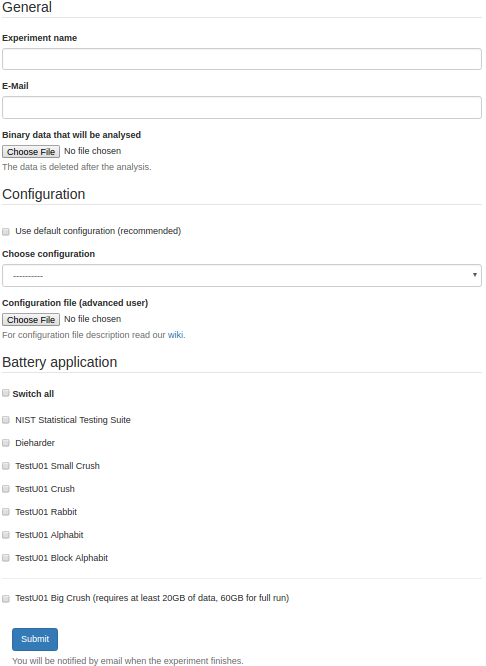
\includegraphics[width=\textwidth+1.2cm]{figures/submit-experiment-form.png} 
\end{nomar}
\end{figure}

\end{document}
